\documentclass[12pt, conference, onecolumn, a4paper]{IEEEtran}
\IEEEoverridecommandlockouts
% The preceding line is only needed to identify funding in the first footnote. If that is unneeded, please comment it out.
\usepackage{cite}
\usepackage{amsmath,amssymb,amsfonts}
\usepackage{algorithmic}
\usepackage{graphicx}
\usepackage{textcomp}
\usepackage{xcolor}
\usepackage{titlesec}
\usepackage{pifont}
\usepackage{soul}
\usepackage{tabularx}
\usepackage[left=1.5in,right=1in,top=1in,bottom=1in]{geometry}

\definecolor{lightcyan}{RGB}{0,255,255}
\definecolor{specBlue}{RGB}{81,0,255}

\def\BibTeX{{\rm B\kern-.05em{\sc i\kern-.025em b}\kern-.08em
T\kern-.1667em\lower.7ex\hbox{E}\kern-.125emX}}

\title{Conference Changes Title}

\author{\IEEEauthorblockN{1\textsuperscript{st} Given Name Surname}
    \IEEEauthorblockA{\textit{dept. name of organization (of Aff.)} \\
        \textit{name of organization (of Aff.)}\\
        City, Country \\
        email address or ORCID}
    \and
    \IEEEauthorblockN{2\textsuperscript{nd} Given Name Surname}
    \IEEEauthorblockA{\textit{dept. name of organization (of Aff.)} \\
        \textit{name of organization (of Aff.)}\\
        City, Country \\
        email address or ORCID}
    \and
    \IEEEauthorblockN{3\textsuperscript{rd} Given Name Surname}
    \IEEEauthorblockA{\textit{dept. name of organization (of Aff.)} \\
        \textit{name of organization (of Aff.)}\\
        City, Country \\
        email address or ORCID}
    \and
    \IEEEauthorblockN{4\textsuperscript{th} Given Name Surname}
    \IEEEauthorblockA{\textit{dept. name of organization (of Aff.)} \\
        \textit{name of organization (of Aff.)}\\
        City, Country \\
        email address or ORCID}
    \and
    \IEEEauthorblockN{5\textsuperscript{th} Given Name Surname}
    \IEEEauthorblockA{\textit{dept. name of organization (of Aff.)} \\
        \textit{name of organization (of Aff.)}\\
        City, Country \\
        email address or ORCID}
    \and
    \IEEEauthorblockN{6\textsuperscript{th} Given Name Surname}
    \IEEEauthorblockA{\textit{dept. name of organization (of Aff.)} \\
        \textit{name of organization (of Aff.)}\\
        City, Country \\
        email address or ORCID}
}

\titleformat{\section}{\normalfont\large\raggedright\MakeUppercase}{\thesection}{1em}{}

\begin{document}
\maketitle
\newpage
\tableofcontents
\newpage
\section{Glossary of terms}

\begin{itemize}
    \item FHS - Frequency Hop Synchronization

    \item ID packers - Identification packets

    \item BLE - Bluetooth Low Energy

    \item UUID - Universally Unique Identifier

    \item TARP - Tiny Ad hoc Routing Protocol

    \item WiFiDi - WiFi Direct

    \item GO - Group Owner

    \item GM - Group Member

    \item LC - Legacy Client
    
    \item POC - Proof Of Concept 

\end{itemize}

\newpage

\section{Introduction}

For many reasons, the need for communication has become one of the most urgent
problems in the modern world. Nowadays, smartphones are almost universally used
as the primary form of communication. Consequently, it would be highly
advantageous if individuals could communicate using smartphones in the absence
of infrastructure. This would eliminate their dependence on infrastructure and
enable them to communicate without infrastructure or provide an alternative to
available infrastructure. There are many well-known smartphone chat
applications, including WhatsApp, Telegram, Viber, and others;
nevertheless, they all depend on the internet and the appropriate communication
infrastructure.

The main infrastructure-based communication methods in smartphones are
cell-based GSM, 4G LTE, and access point-based WiFi, and assorted technologies.
But when it comes to an infrastructure-less environment, the nodes do not have
to connect to the
cellular towers since they establish direct wireless connections. In this case,
the ability to leverage various infrastructure-free communication protocols is
referred to as being adaptive. Thus, mobile ad-hoc networks are networks
created dynamically without the need for infrastructure, presuming that all
nodes connecting to the network will be portable to some
extent\cite{chlamtac2003}.

Wi-Fi (in ad-hoc mode) and Bluetooth come out on top regarding available
infrastructure-less communication methods. Bluetooth is one of the most popular
short-range wireless technologies for transferring data between devices over
short distances. It took the place of the conventional cable connections that
were used to transport data between our regularly used portable gadgets. When
compared to Wi-Fi, Bluetooth is less expensive and uses less power, but Wi-Fi
offers more benefits, such as faster speeds and broader transmission ranges.
Although Wi-Fi's ad hoc mode could handle direct device-to-device (D2D)
communication without needing an Access Point (AP), this requires rooting of
the device in Android smartphones\cite{soares2017}. On the other hand, Wi-Fi
Direct (Wi-Fi P2P), which is
constructed on top of the infrastructure mode of Wi-Fi, enables simple and
effective D2D communication and lets the devices choose who will take over the
AP-like functions. Another technology to consider is Bluetooth Low Energy
(BLE), a development of Bluetooth that significantly reduces battery usage
because it establishes brief connections and stays in sleep mode when not
connected.

Factors that need to be considered when developing a framework for
infrastructure-less communication in mobile devices are affordable power
consumption, message transmission dependability, message delays, routing
mechanism performance, and network establishment speed in
different scenarios. Also, the topology of mobile ad
hoc networks frequently changes due to factors including node mobility and
unexpected node unavailability.

Due to this, it is crucial to find appropriate routing methods and neighbor
identification techniques to increase communication effectiveness in these
kinds of networks.

Meshify is a framework for infrastructure-less communication using smartphones.
It is currently equipped only with Bluetooth classic and BLE
technologies\cite{gunasekara2022}. Implementing Wi-Fi Direct as an additional
wireless communication technology for Meshify will significantly enhance its
connectivity capabilities. Wi-Fi Direct offers faster data transfer speeds and
a more stable connection than Bluetooth, making it ideal for real-time data
exchange applications, as explained above. This expansion will empower Meshify
with a versatile and robust communication framework, improving its performance
and usability. Also, improvements should focus on improving the current Meshify
neighbor discovery protocol for accurate device detection and multi-hop message
relaying to extend network reach. Incorporating research from opportunistic
networks can enhance communication resilience. In addition, the Meshify
middleware framework should adhere to the best software engineering principles
and design patterns to ensure that third-party app developers may readily use
it.


\section{Problem Statement}

In the absence of networking infrastructure, smartphones fail to deliver
network services. The available solutions for infrastructure-less communication
are limited in terms of the underlying communication technologies and
limitations imposed by operating systems.

\section{Research Objectives}

\begin{itemize}
      \item Develop a modular application layer framework to enable ad hoc
            networking in
            Android smartphones with Bluetooth, Bluetooth Low Energy, and WiFi Direct
            as
            communication methods.
      \item Develop a prototype chat application with filesharing capabilities
            implementing
            the developed framework.
      \item Simulate reactive routing protocols with mobility models and
            identify suitable
            protocols for a typical mobility model.
\end{itemize}


\section{Literature review}

The core feature that sets ad hoc networks apart from conventional networks is
the need for no infrastructure to create and maintain the network. In an ad hoc
network, the nodes act as network relays, eliminating the need for established
infrastructure. Due to these factors, ad hoc networks are extensively used in
sensor networks and other IoT-related domains\cite{akyildiz2002}. Another
instance where infrastructure-less networks become useful is in times of
disaster and defense scenarios, where existing infrastructure may be
unavailable or unreliable. In such cases, ad hoc networks can aid in
maintaining networks confined to vehicles and other mobility units and can aid
in critical communications in disaster scenarios, even forming part of a
corporate data backup system\cite{raza2016}.  However, in recent years,
consumer use of smartphones skyrocketed. The global smartphone usage is
estimated to be 6.92 billion, roughly 86\% of the world population in
2023\cite{zippia2023}. This availability makes smartphones an ideal device for
consumer-level general-purpose ad hoc networking\cite{soares2017}.

Since the foremost need among users of mobile devices is
connectivity\cite{chlamtac2003}, mobile devices in self-configured,
self-maintained networks delivering network connectivity where no connection
infrastructure is present is highly desirable\cite{chlamtac2003}. Apart from
intra-network communication, Mobile Ad Hoc Networks can also share internet
service via an access point, effectively extending the Internet service
area\cite{chlamtac2003}.

While the use of ad hoc networks for IoT and sensor-based applications is
well-established, the same implementations can not be applied to consumer
mobile devices due to limitations imposed by the operating systems and network
implementations of mobile devices.

\subsection{Ad Hoc Networking Frameworks for Android}

This section aims to establish the current state of the art on Android
frameworks and implementations aiming to facilitate ad hoc network
capabilities.

The Serval Project introduces an application that creates self-managed meshable
networks using the Wi-Fi interfaces of the devices\cite{gardner2013}. The
Serval system also supports a mesh extender\cite{gardner2013}. This
air-droppable UHF packet radio extends the mesh network's service range, making
it suitable for providing stable networks where infrastructure is not present -
extending the initial use case of disaster management. However, since the
Serval mesh is a standalone application and is not a framework available to use
by programmers.

Bluetooth and Bluetooth Low-Energy connectivity are also used to create
proximity-based communication networks. Wang et al. propose a  framework and a
proof of concept chat application using Bluetooth and
Wi-Fi-direct\cite{wang2015}. Since each device carries two unique identifiers
for Bluetooth and Wi-Fi-direct, the system uses a device serial number for
identification. The routing is done with a simple flood-based routing protocol,
and each node reads and floods each received message\cite{wang2015}. Therefore,
the accompanying proof of concept application does not support private
messages. Moreover, the framework assumes that Bluetooth master devices and
WiFi-Direct Group Owners are up and available before the clients are connected.
Therefore, the framework is not easy to use in real-world scenarios as in
MANETs due to node mobility, the topology changes rapidly, and in the case of
WiFi Direct, if the group owner is disconnected, the group will be discarded
and recreated\cite{raza2016}. The framework proposed by Wang et al. is not
resilient to these conditions\cite{wang2015}.

Meshrabiya\cite{meshrabiya} is another framework utilizing the core networking
features of the Android operating system. The framework uses the Wi-Fi Direct
(WiFiDi) standard to create and maintain an ad hoc network with
WiFiDi-compliant and legacy devices. The framework achieves this by maintaining
multiple groups with fully qualified Group Owners and legacy hotspot mode
devices. For routing, the framework uses the link-local IPV6 addresses.
However, as mentioned in the framework documentation\cite{meshrabiya}, there are
limitations in devices running Android versions higher than 11 due to the
access point concurrency feature. Moreover, since the only communication method
available in the framework is WiFi, the usability of the framework is reduced.
Also, another notable factor is that the implementation requires a QR code to
be scanned for inter-group routing.  A more modular framework where the
application programmers can select the communication method as needed will
increase the framework's usability.

Bridgefy\cite{bridgefy} is another framework implemented to be a
programmer-friendly implementation of mesh networks using Android smartphones.
While the Bridgefy framework supports iOS and Android devices with universal
compatibility, the framework only employs Bluetooth as the communication
technology.

The above findings are summarized in table~\ref{litreviewMatrix} for ease of reference.

As evident by the literature review, there is ample opportunity for developing
a general application framework that allows programmers to access networks in a
generalized manner. Since the framework must be application or
scenario-agnostic, the routing algorithms must be chosen based on a generalized
mobility model.

\begin{table}[htbp]
    \centering
    \begin{tabularx}{\textwidth}{|X|X|X|X|X|X|X|}
        \hline
        \textbf{Reference} & \textbf{Accessible Framework} & \textbf{Autonomous Setup and Repair} & \textbf{Open Source} & \textbf{WiFi-Direct} & \textbf{Bluetooth or BLE} & \textbf{Rooting or modification to OS is not needed}\\ \hline
        Meshify\cite{gunasekara2022} & \checkmark & \checkmark & \checkmark & \ding{55} & \checkmark & \checkmark \\ \hline
        Bridgefy\cite{bridgefy} & \checkmark & \checkmark & \ding{55} & \ding{55} & \checkmark & \checkmark \\ \hline
        Meshrabia\cite{meshrabiya} & \checkmark & \ding{55} & \checkmark & \checkmark & \ding{55} & \checkmark \\ \hline
        Serval Project\cite{gardner2013} & \ding{55} & \checkmark & \checkmark & \ding{55} & \checkmark & \checkmark \\ \hline
        Wang et al.\cite{wang2015} & \ding{55} & \ding{55} & \ding{55} & \checkmark & \checkmark & \checkmark \\ \hline
        \textbf{This Project} & \checkmark & \checkmark & \checkmark & \checkmark & \checkmark & \checkmark \\ \hline 
    \end{tabularx}
    \caption{Comparison of existing frameworks}
    \label{litreviewMatrix}
\end{table}

\subsection{Routing Protocols}

Proactive routing protocols that seek out nodes and maintain a routing table
are not suitable for routing ad hoc networks due to the highly mobile nature of
the nodes. As nodes move in and out of the network coverage area, the network's
topology is altered, outdating the gathered routing information. Therefore, the
suitable routing protocols are reactive\cite{reina2011}. Raza et
al.\cite{raza2016} analyze several different protocols for different network
traffic and connection types using metrics such as throughput and end-to-end
delay.

The following sections explain some widely studied routing protocols in ad hoc
networks.

\subsubsection{Simple Flooding}

Flooding is one of the most basic routing methods used in MANETs since
broadcast forwarding is the main method of operation in many wireless
networks\cite{chlamtac2003}. In MANETs, this involves nodes forwarding every
incoming packet to all the neighbors within its range. However, this is not
ideal as with the increase of the size of the network, flooding can create
broadcast storms and decrease network availability\cite{chlamtac2003}.

\subsubsection{Ad hoc Demand Distance Vector (AODV) }

AODV is a reactive routing protocol allowing unicast routing. When a node needs
to send a packet to another node, it sends an RREQ packet mentioning the
required destination node\cite{reina2011}. The neighboring nodes forward the
RREQ packet until it reaches the destination node, and RREP is sent by the
destination node and is doubled back to the source, enabling the source to
route the data packet to the destination node\cite{reina2011}.

\subsubsection{Dynamic Source Routing(DSR)}

In DSR, instead of depending on the nodes to handle routing, the complete path
to the destination node is sent with the RREP packet in the header to the
source node\cite{chlamtac2003}.

As found by Reina et al. with simulated node mobility models, AODV performs
better than other routing protocols\cite{reina2011}.


\section{Methodology}

As revealed in the literature review, there is a gap in a general-purpose
networking framework in smartphone-based ad hoc networking. The existing
implementation of the framework partially fills the gap. However, the current
framework only uses Bluetooth Classic and Bluetooth Low-Energy technologies to
communicate. This can be improved by using Wi-Fi Direct technology. Moreover,
the routing algorithm used in the current framework can be further enhanced
after research on the performance of routing algorithms. In the following
sections, the core technologies used will be discussed.

\subsection{Modular Framework}

Our objective is to enhance the existing implementation by introducing a
modularized framework while also striving to incorporate WiFi Direct
functionality. This improved framework will continue to serve as a versatile
platform for sharing text messages among network nodes and will subsequently be
extended to facilitate seamless media and file transfers.

The previous implementation was primarily centered around Bluetooth Classic and
BLE technologies, allowing us to address a specific range of communication
needs. In this upgraded version, we aim to diversify the connectivity options
by exploring the capabilities of WiFi Direct. This will enable us to harness
the benefits of high-speed communication over Wi-Fi connections, complementing
the existing Bluetooth functionalities.

By modularizing the framework, we intend to enhance its flexibility and
scalability, making it easier to customize and adapt to different applications
and use cases. This approach will facilitate the integration of new Transport
modes other than the ones mentioned.

The following figure~\ref{figArch} shows a high-level diagram of the upgraded
framework. A brief description of the components is given below.

\begin{itemize}
    \item \textbf{MeshifyClient:} This behaves as an entry point for
          application programmers.
    \item \textbf{DiscoveryManager:} Used in the neighbor discovery process
          using the implemented neighbor discovery protocol
    \item \textbf{ConnectionManager:} Manages device connections
    \item \textbf{FowardController:} Manages message passing in multihop
          communication
    \item \textbf{TransportManage:} Manages the communication between the
          Android layer and the framework based on the Transports in a modular
          way.
\end{itemize}

\begin{figure}[htbp]
    \centerline{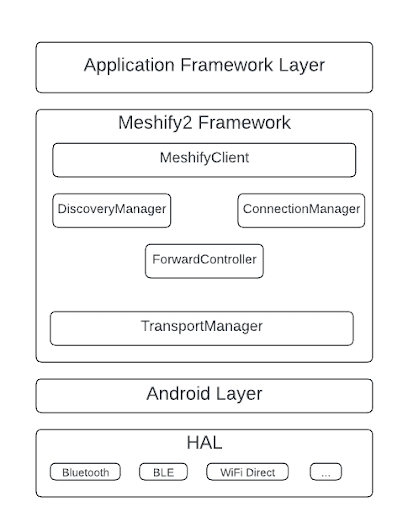
\includegraphics[height=0.45\textwidth]{imgs/classArch.png}}
    \caption{Upgraded Framework}
    \label{figArch}
\end{figure}

\subsection{Bluetooth and Bluetooth Low Energy}

\subsubsection{Bluetooth Classic}

In classic Bluetooth, an inquiry device transmits inquiry packets called
identification packets(ID packets) and listens to inquiry responses called FHS
(Frequency Hop Synchronization) packets. The neighboring devices must be in an
inquiry scan to receive ID packets and reply with FHS packets. ID packets give
no information about the inquiry device. But FHS packets have the Bluetooth
address and other information about the responding device. Also, the inquiry
process does not establish any connection. Connection is established in the
page procedure where a device responds in its page scan procedure to the device
that carries out the paging. This paging is only targeted for a single device
identified in the inquiry process. The paging device is considered the master
device for the connection. Responding devices are the slaves, and every device
can become a slave or a master, and the roles can be switched within a
connection. Piconet is the basic Bluetooth topology, which consists of a master
and slaves, and the active slaves for a master should be seven or fewer. A
Bluetooth scatternet consists of more than one piconet. As explained in
neighbor discovery protocols, they can be categorized as direct and indirect.
Only the immediate neighboring nodes are discovered in the direct method, and
in the indirect method, nodes can learn about other existing nodes through
their neighboring nodes\cite{todtenberg2019}.

In the Meshify Framework, a Bluetooth device can act as both a client and a
master, and each role has its thread to do so\cite{gunasekara2022}. One thread
is set as discoverable for incoming connections, while the other thread
performs scanning. Also, the Bluetooth discovery protocol allows the devices to
be connected without pairing.

\begin{figure}[htbp]
    \centerline{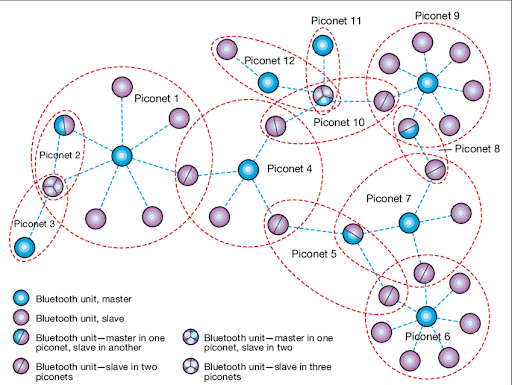
\includegraphics[height=0.45\textwidth]{imgs/piconetbl.png}}
    \caption{Bluetooth Scatternet Diagram consisting of several piconets
        \cite{Larsson2000}}
    \label{piconetbl}
\end{figure}

\subsubsection{Bluetooth Low Energy}

‘Scanners ’ listen for advertising events actively broadcasted by ‘Advertisers’
over the physical channels. Since the scanners can initiate a connection after
receiving from an Advertiser, they are also called “Initiators.” After the
advertiser accepts the connection request, the scanning device becomes the
master, and the advertising device becomes the slave. Also, the BLE
specifications don't limit the number of slaves. In Piconet, they don’t use a
shared frequency channel, and the master gives a unique hopping sequence
point-to-point for each slave. So the master uses the polling technique to
communicate with its slaves consecutively using time division multiplexing
\cite{todtenberg2019}.

\begin{figure}[htbp]
    \centerline{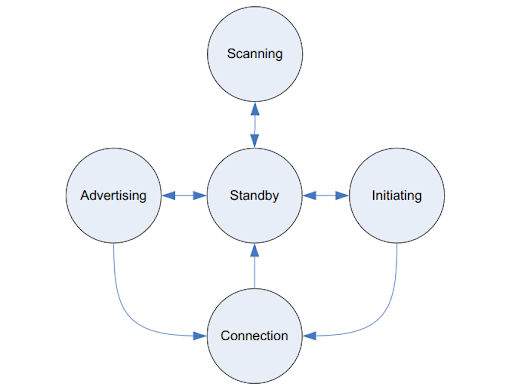
\includegraphics[height=0.45\textwidth]{imgs/blstatemach.png}}
    \caption{BLE State Machine}
    \label{blstatemach}
\end{figure}

\subsubsection{Neighbor Discovery Process for Meshify}

When a client connects with the master, the client sends a handshake packet
containing its Meshify UUID. Master adds the client to its neighbor devices
list and sends the handshake ack containing its UUID and the neighbor list. So,
the client adds the master and the neighbor list to its neighbor list. Since
when a client sets a connection with the master, all the other clients should
know about the new client, the master responds with a
broadcast\cite{gunasekara2022}.

\begin{figure}[htbp]
    \centerline{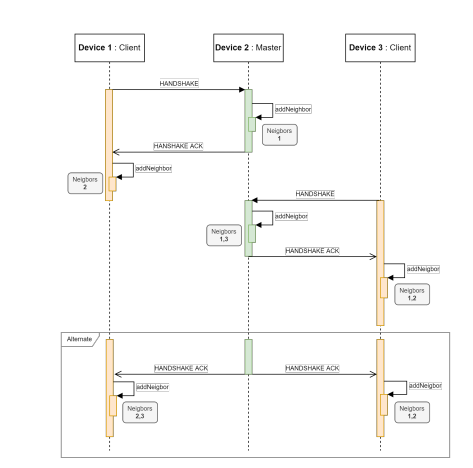
\includegraphics[height=0.75\textwidth]{imgs/neighbourdis.png}}
    \caption{Neighbour Discovery Process for Meshify\cite{gunasekara2022}}
    \label{neighbourdis}
\end{figure}

\subsubsection{Routing for Meshify}

Meshify utilizes TARP, a simple routing protocol, to route traffic via a
controlled flooding method. TARP is a layer-less routing scheme that was
created for Wireless Sensor Networks. The protocol is a set of rules a node
must follow to process each packet\cite{gunasekara2022}. According to
\cite{wsn2021} in TARP, unless there is a specific reason not to do so, a node
floods the packet to all surrounding nodes.

\begin{figure}[htbp]
    \centerline{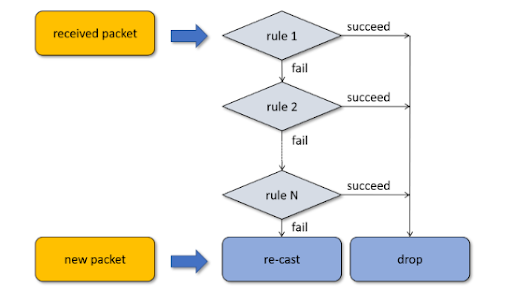
\includegraphics[height=0.45\textwidth]{imgs/tarpproc.png}}
    \caption{The mechanism of TARP \cite{wsn2021}}
    \label{tarpproc}
\end{figure}

As seen in Fig.~\ref{tarpproc}, the rules will be implemented in the order
listed, beginning with rule number 1 and progressing to the last rule. If a
specified rule is met, the packet is dropped. Following a rule implies
determining a reason to drop the packet. A rule can examine the full packet of
data being transmitted and use any criteria it desires to determine what to do
with that data. This rule can receive the packet, change what's inside, or
generate a new delivery packet. Some rules have specific expectations about
what is in the packet, and the application employing these rules can adapt them
to meet its particular requirements\cite{wsn2021}.

Gburzyński\cite{wsn2021} discusses some main rules used in TARP.

\begin{itemize}
    \item Limit Hop Count (LHC) - This rule restricts the number of hops a
          packet can take. Following the creation of a packet by a source, the
          number of
          forwardings to which the packet was subjected is counted, including
          the initial
          transmission. When the number of hops for a specific packet reaches
          the
          maximum, the packet is dropped.

    \item Duplicate Discard (DD) - This rule attempts to prevent the same
          packet from being sent numerous times. Each packet contains a unique
          identifier
          known as a serial number. When a node forwards a packet, it stores a
          signature
          that is a combination of the sender's address and the packet's serial
          number.
          If the node already possesses the signature, the packet will be
          dropped because
          it has previously been delivered through this node.

    \item Sub-optimal Path Discard (SPD) - Using the rule DD, a node listens to
          another node delivering a packet and determines the shortest number
          of hops to
          reach that node. Assume an intermediary node exists between the
          sender and
          destination nodes. The intermediate node has the fewest hops from the
          sender to
          that node and from that node to the destination. If the sum of the
          hops is
          larger than the smallest number of hops from the sender to the
          destination
          node, the packet will bypass the intermediate node.

\end{itemize}

All of the TARP rules outlined above govern the flooding process for Meshify.
Aside from the TARP restrictions, the Meshify has single-hop acknowledgments to
improve reliability. However, because this can reduce throughput, only the
packet's destination sends single-hop acknowledgments to its
neighbors\cite{gunasekara2022}.

\subsection{Wifi-Direct}

Wi-Fi Direct is a P2P communication standard complying with the IEEE 802.11
standard. The core purpose of the standard is to enable WiFi-enabled mobile
devices to connect to printers and other WiFi-enabled devices in a peer-to-peer
manner\cite{malar2023}.

Compared with the Bluetooth and Bluetooth Low Energy standards described above,
WiFi Direct as a communication method has two main advantages.

\begin{itemize}
    \item Speed: As Malar et al. present, WiFi connections have a speed greater
          than 54Mbit/s while Bluetooth speed is limited to 3 Mbit/s. This is
          advantageous in facilitating fast file transfer.

    \item Security: WiFi Direct uses the WPA2 standard, which is more secure
          for data transfers than Bluetooth.
          Therefore, implementing a multi-hop ad hoc network using WiFi Direct
          is
          advantageous.

\end{itemize}

\vspace{0.3cm}

\subsubsection{Operation of Wifi-Direct}
WiFi Direct (WiFiDi) is primarily a P2P standard operating in a functional
structure called a Group. A group consists of a Group Owner and a set of P2P
clients (referred to as a Group Member) that connect as peers to the Group
Owner. In WiFiDi, the roles of the devices, whether a P2P client or a Group
Owner (GO), are not predetermined but negotiated at group formation.

Only devices conforming to the standard are equipped to participate in the
group formation procedure. However, once the group is established, devices
without WiFiDi can connect to the GO as an ordinary WiFi
client\cite{funai2015}\cite{wifidispec}. This case can be referred to as a
Legacy Client.

\begin{figure}[htbp]
    \centerline{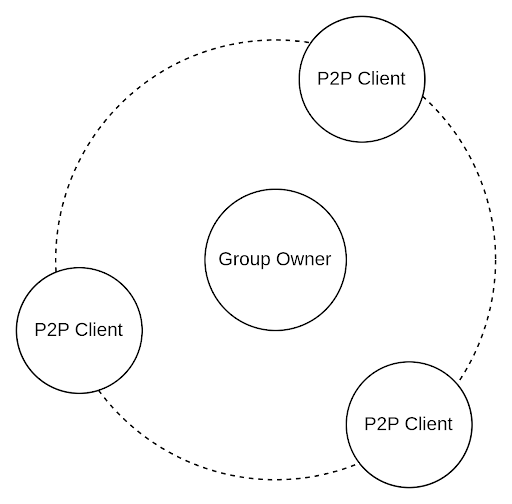
\includegraphics[height=0.45\textwidth]{imgs/group.png}}
    \caption{A WiFi-Direct Group}
    \label{digroup}
\end{figure}

\subsubsection{Group Formation Procedure}

Before the group formation begins, all devices not currently in a WiFiDi group
are put into a listen state where the devices listen in a given “listen
channel”; this channel is selected from the “social channels” set. In the
2.4Ghz band the list of social channels is 1, 6, and 11\cite{wifidispec}. Once
devices are discovered they move to the group formation phase.

There are two main stages of group formation and three main modes of group
formation the nodes can be configured to follow. The following section
describes the standard group formation action flow.

\begin{enumerate}
    \item Group owner negotiation

          Considering the case of two devices performing a negotiation, a
          handshake of three frames is implemented by the standard. Each frame
          contains
          the device information, P2P capabilities and owner
          intent\cite{wifidispec}.
          Owner intent is a metric of the device’s intent of becoming a group
          member. This process is outlined by Fig.~\ref{formproc}
          %add the thing here

    \item Provisioning

          The provisioning step sets up the group following the WiFi Protected
          Setup\cite{wifidispec}, allowing the group members to share data in
          secure
          sessions.

\end{enumerate}

\begin{figure}[htbp]
    \centerline{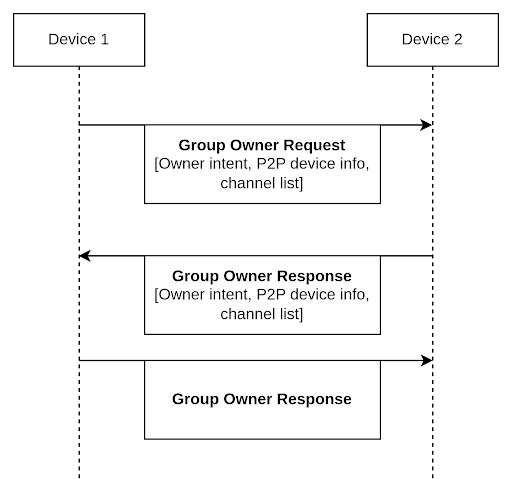
\includegraphics[height=0.45\textwidth]{imgs/formproc.png}}
    \caption{Standard WiFi Group Formation Procedure}
    \label{formproc}
\end{figure}

\subsubsection{Intra-Group Routing}

After the group owner is established and the group is provisioned, the group
owner acts as a DHCP host to provide IP addresses to each peer in the
group\cite{funai2015}. The group owner then acts as a Soft-Access Point and
controls routing between nodes within the group and other network operational
and management functions such as channel management\cite{wifidispec}.

\subsubsection{Inter-group routing (Multi-hop Routing)}

As mentioned above, the WiFiDi standard ensures P2P communication between the
Group Owner and the Group Members, and by the soft-AP role of the Group Owner,
the routing within the group. However, the standard does not provide any
mechanism for multi-hop routing.

However, there are two possible ways of achieving this. All two methods involve
a gateway node, either temporarily or permanently connected to more than one
group. The simultaneous connection of a single node to two different groups is
not excluded in the standard. However, the functionality of such an arrangement
may depend on the specific implementation of the standard\cite{funai2015}.

According to Funai et al., the gateway can be either a group member or legacy
client of either group and in the second scenario, the gateway node can also be
a group owner in one and a group member or a legacy client in the second
group\cite{funai2015}.

However, it is impossible to directly implement these strategies due to the
Android operating system limitations.

For example, as observed by Funai et al., when the gateway node is a group
member of one group and a legacy client of the other group, the gateway could
receive packets from both groups. Still, it could not send outgoing packets to
either\cite{funai2015}.

Funai et al.\cite{funai2015} presented two mechanisms to overcome this.

\begin{enumerate}
    \item A timeshare mechanism
          As presented in Fig~\ref{timeshare}, this mechanism, the gateway node
          can
          disconnect from the source group
          and dynamically connect to the destination group at packet transfer.
          The
          Android APIs do not supplement the switching process and must be
          handled at the
          application level\cite{funai2015}.
    \item Simultaneous connection
          Authors found that it is possible to use the gateway node as a group
          member
          in one group and a local client in the other to transfer data using
          the UDP
          multicast socket supplied in Android\cite{funai2015}.
\end{enumerate}

\begin{figure}[htbp]
    \centerline{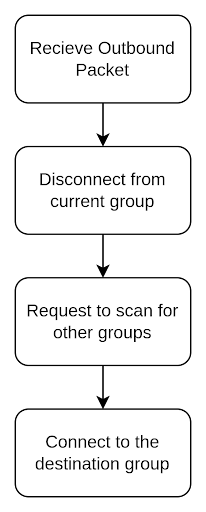
\includegraphics[height=0.45\textwidth]{imgs/timeshare.png}}
    \caption{Gateway Node Timeshare Procedure}
    \label{timeshare}
\end{figure}

\vspace{0.3cm}

\subsubsection{Android SDK and WiFi Direct}
The main WiFi Direct functionality in Android is provided by the WiFiP2pManager
class in the Android SDK. This class allows for the complete group creation and
other related operations in the WiFiDi standard.

Following are the core methods in WiFi Direct implementation\cite{wifiman}.

\begin{itemize}
    \item discoverPeers(): Discover available peers
    \item createGroup(): Initiate the group creation mechanism
    \item removeGroup(): Remove the currently connected group
    \item requestGroupInfo(): Request for the connected group info
\end{itemize}

\vspace{0.1cm}

This API can create an application layer framework capable of performing
inter-group(multi-hop) routing.

\subsection{Simulations and Testing}

It is vital to test the proposed framework and the applications during and
after the development process to ensure that the network traffic is handled
properly at different levels of traffic and mesh scenarios. Morote et al.
provide a mechanism for testing routing protocols with the open-source software
module called Network Simulator 2\cite{morote2010}. The newest version of
Network Simulator is version 3, commonly known as ns-3\cite{ns3}. Ns-3 is a
discrete event simulation platform written in C++ and it supports OTcl scripting
language for modeling node mobility\cite{morote2010}. However, our simulation
scenario is different from the standard testing scenario for ns-3 due to the
fact that the routing and other features are handled on the application layer.

Another simulation platform available is the OMNET++ simulation platform. The
platform allows simulating nodes and network event behaviors using C++ classes
and also provides an IDE and a graphical simulator runner\cite{opensim}. We aim to
use this platform to simulate the framework and test under different mobility
scenarios.

Therefore, we aim to simulate the framework on the ns3 platform and test under
different scenarios of node availability and mobility.

\vspace{0.3cm}

\subsubsection{Simulation Plan}
The existing simulations and results will be extended by adding the following
specifications and analyzing the results.

\vspace{0.3cm}

Comparative routing protocols:
\begin{itemize}
    \item TARP
    \item AODV
    \item DSDV
\end{itemize}

\vspace{0.3cm}

Mobility Models:
\begin{itemize}
    \item Gauss-Markov Mobility Model
    \item Manhattan Grid Model
\end{itemize}





\section{Discussion}
\subsection{Current Progress}
\subsubsection{Network Simulation}

Simulation of AODV protocol for static and Gauss-Markov mobility is completed.
Due to updates to the OMNET++ simulation environment and the INET framework,
the earlier implementation of the TARP protocol is incompatible with the latest
versions. Therefore, necessary adaptations are being carried out.

\begin{figure}[htbp]
    \centerline{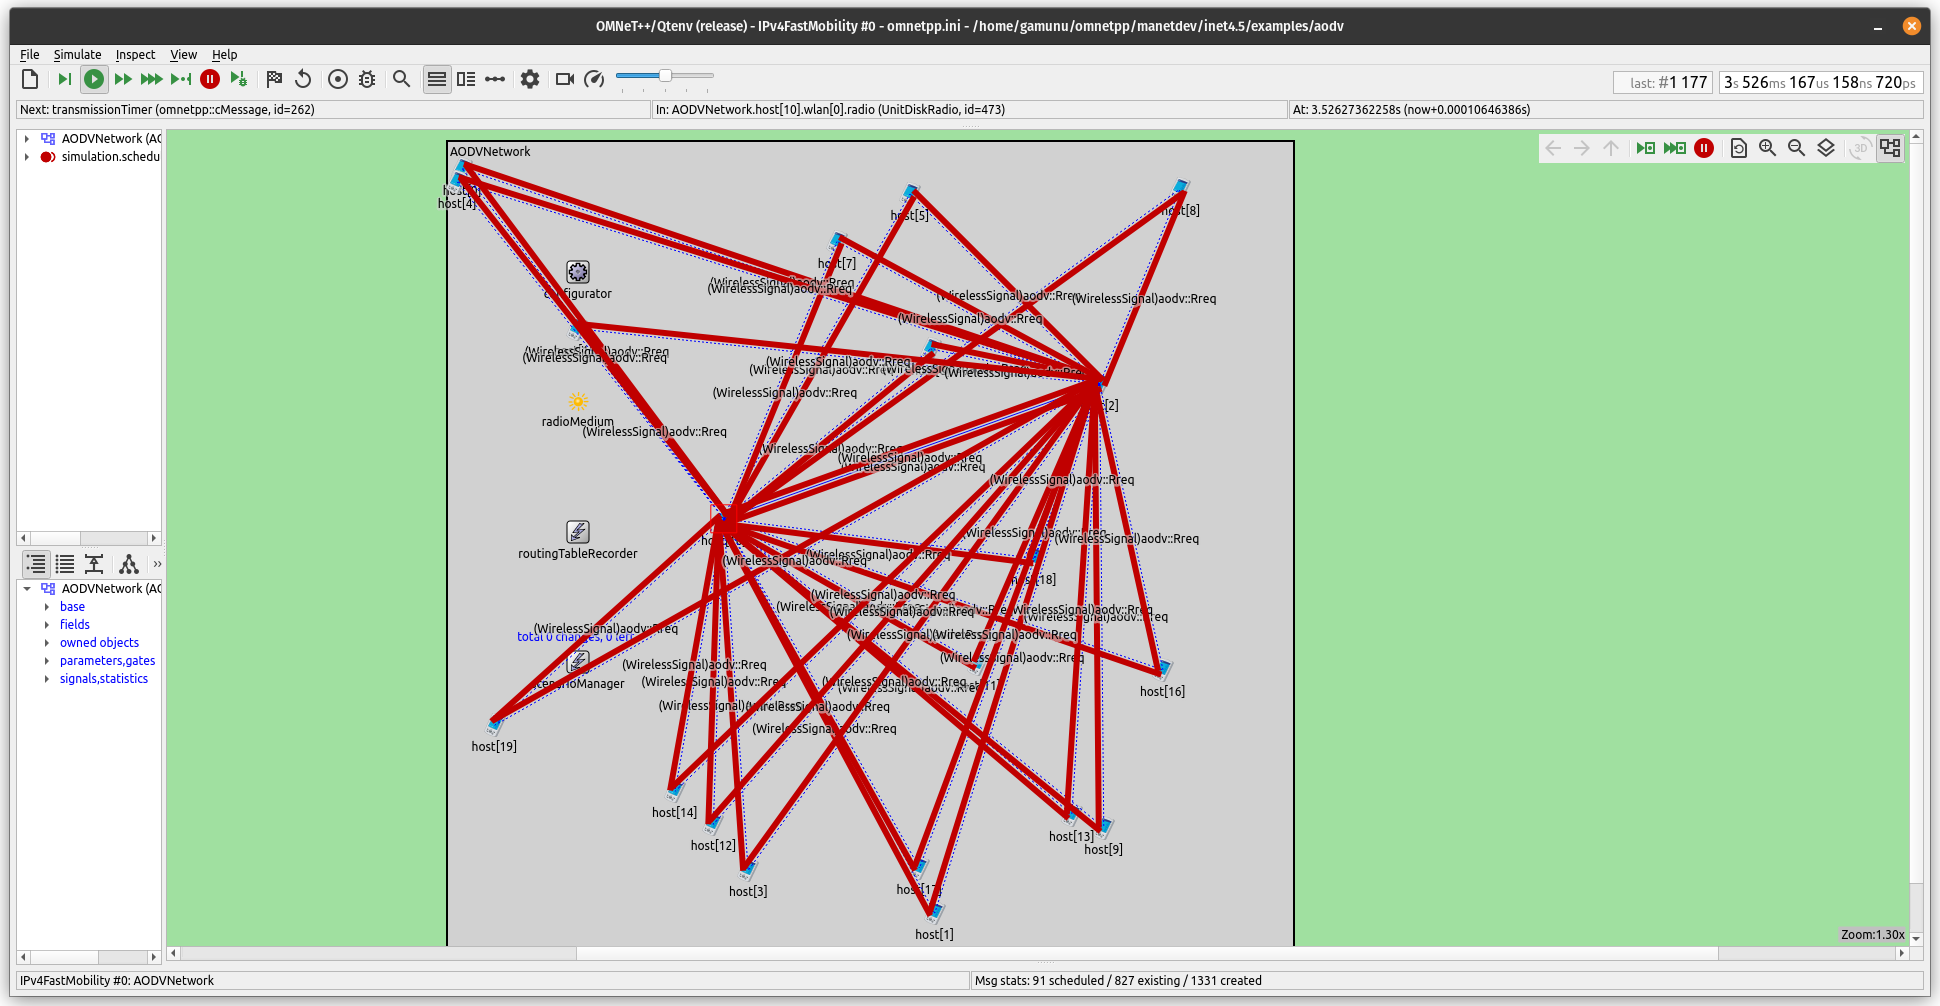
\includegraphics[height=0.45\textwidth]{imgs/aodvSim.png}}
    \caption{AODV protocol network simulation}
    \label{aodvSim}
\end{figure}

\subsubsection{WiFi Direct POC}

To test the feasibility and refine the implementation method, we have developed
a POC application for using WiFi Direct as a communication method. Currently,
communication among clients of the same group is implemented. The group
formation is handled by \texttt{WifiP2pManager}, provided by the Android
SDK\cite{wifiman}.

\vspace{0.3cm}

\paragraph{POC App Implementation}

The POC application sets up a WiFi Direct group, and once the group is
established, allows sending text messages within the created group, both
between Group Members and between Group Owner and Group Members.

The figure~\ref{labelewifidipoc} shows a labeled interface of the developed POC
application.

\begin{figure}[htbp]

    \centerline{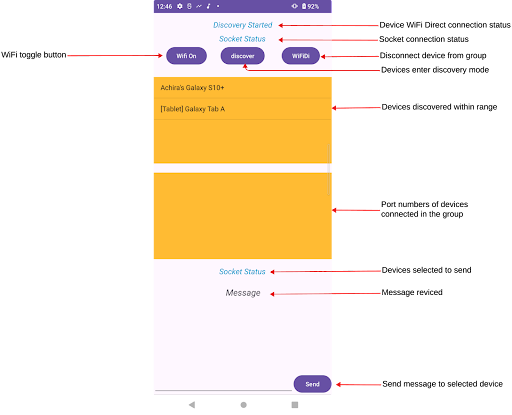
\includegraphics[height=0.9\textwidth]{imgs/labledwifidipoc.png}}
    \caption{Labled interface of the POC application.}
    \label{labelewifidipoc}
\end{figure}

Once the nearby WiFi Direct-enabled devices are discovered, the devices perform
a group owner negotiation and establish a WiFi Direct group. Once the group is
established, the Group Owner(GO or Host, as referred to in the POC application)
can communicate with the sockets connected to each device in the group.

Once this stage is reached, each client can view the host or Group Owner's
device name in the discovery list. The group owner can view the clients
connected to it. This is demonstrated in Figure~\ref{group}.

\begin{figure}
    \centering
    \begin{subfigure}[b]{0.3\textwidth}
        \includegraphics[width=\textwidth,
            height=0.4\textheight]{imgs/hostaftergroup.png}
        \caption{Host interface after creating a group with one client.}
        \label{group:host}
    \end{subfigure}
    \hspace{1cm}
    \begin{subfigure}[b]{0.3\textwidth}
        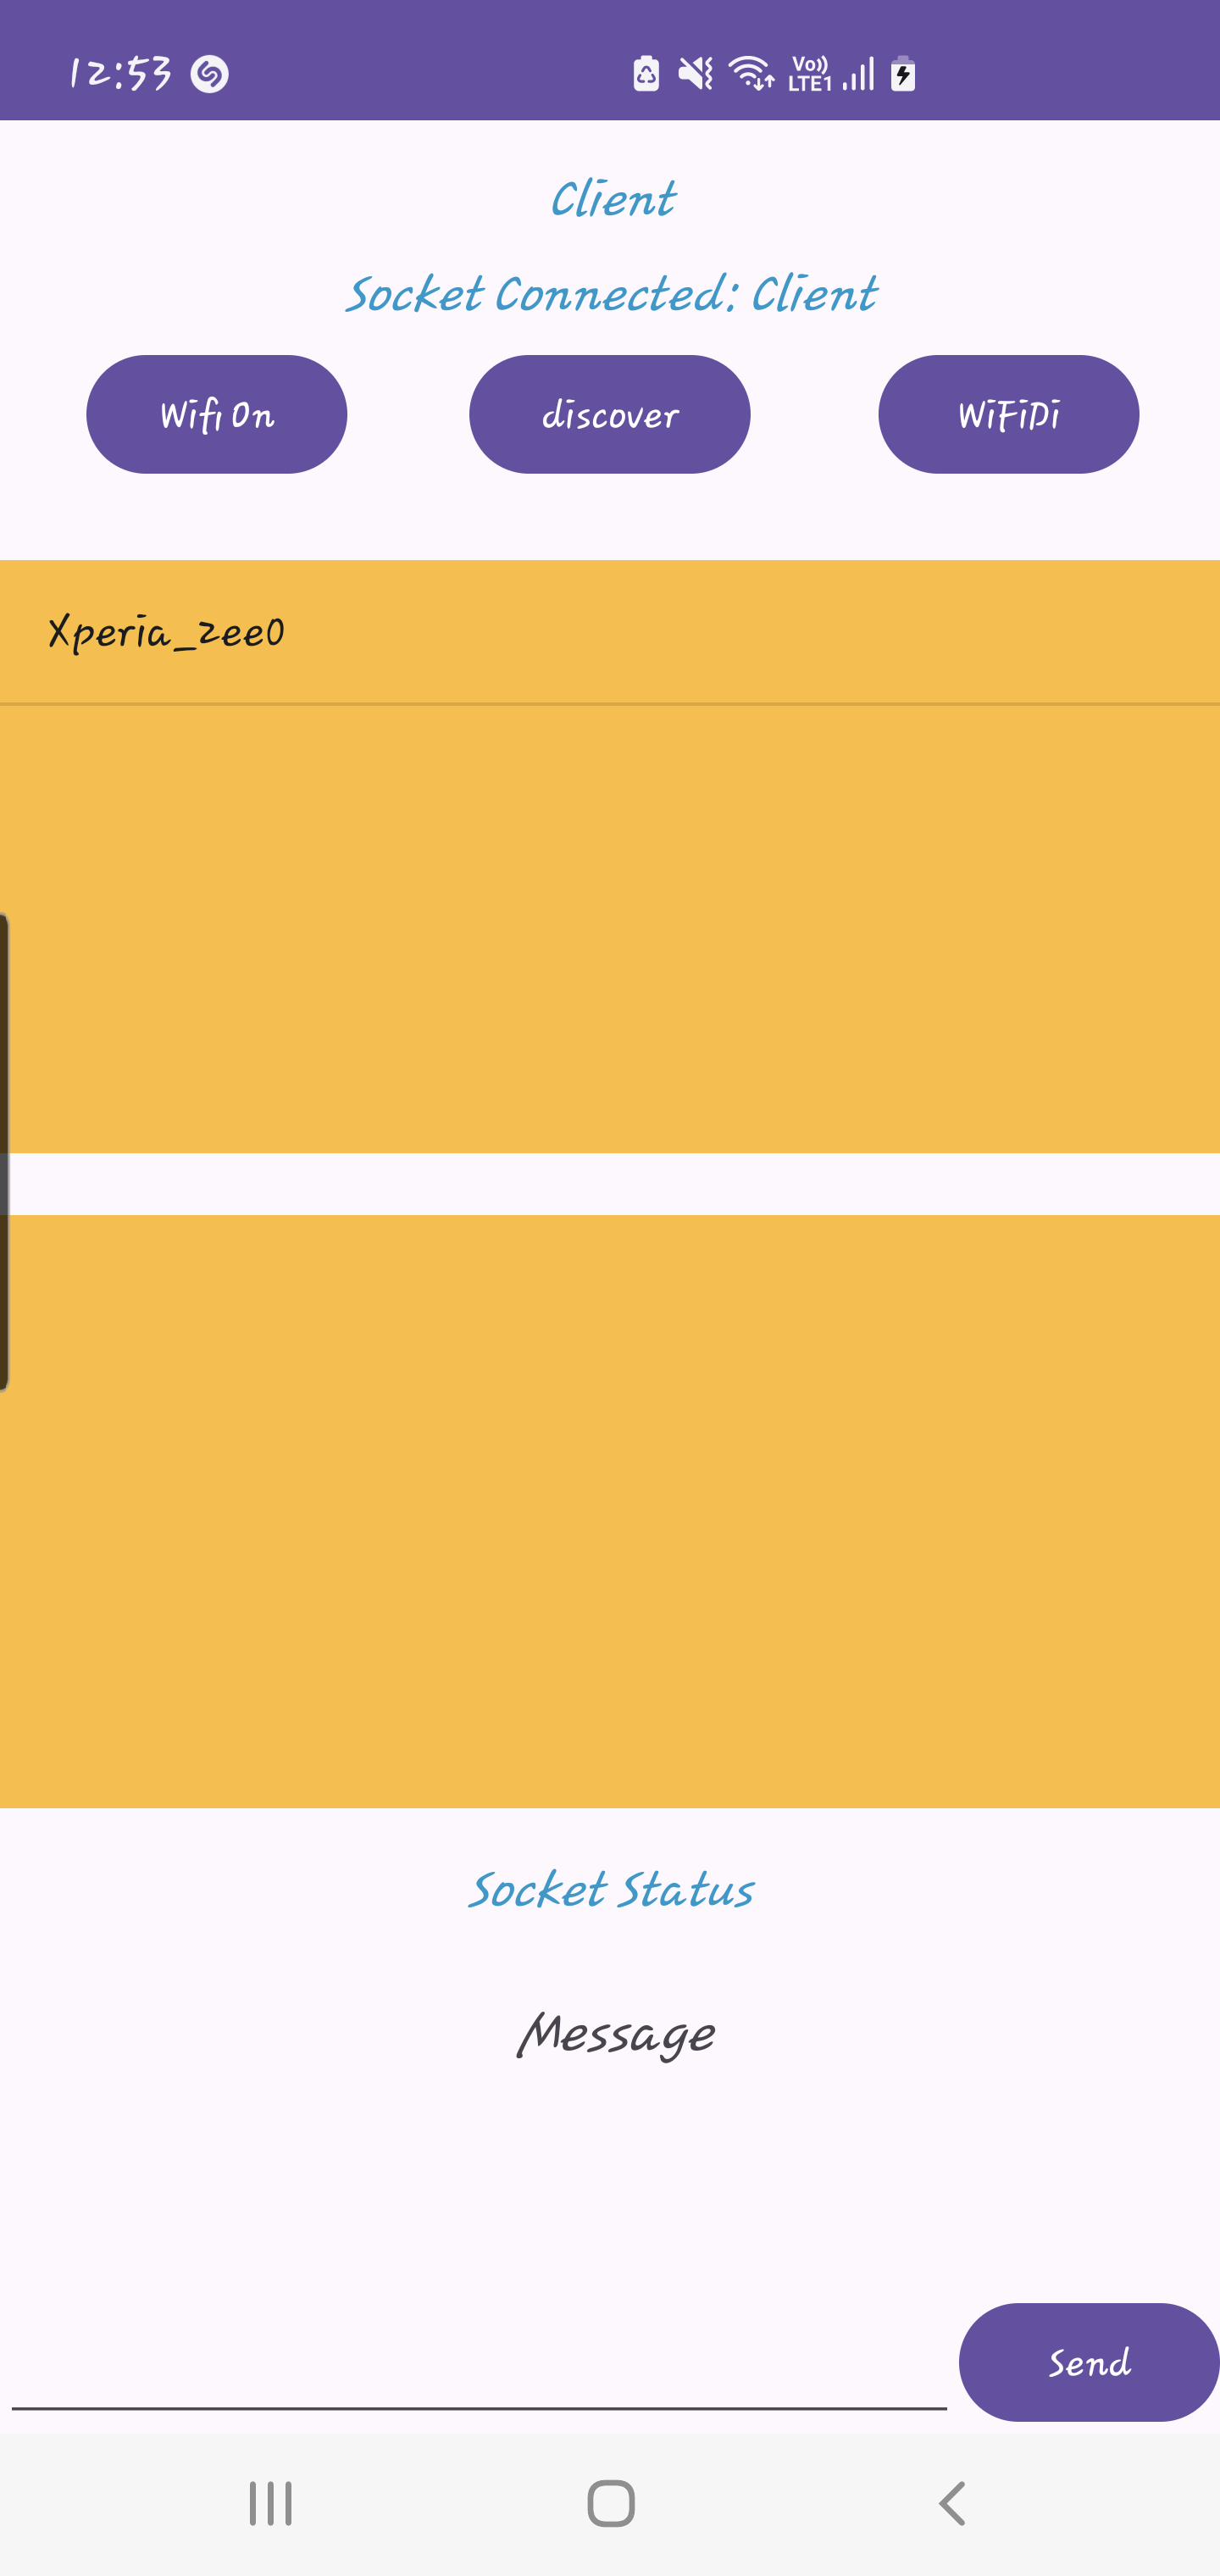
\includegraphics[width=\textwidth,
            height=0.4\textheight]{imgs/clientAfterDiscovery.png}
        \caption{Client interface after a group is created.}
        \label{group:client}
    \end{subfigure}
    \caption{Caption for the whole figure.}
    \label{group}
\end{figure}

After a group is created, communication between the host and client are
possible as demonstrated by the Figures~\ref{clientComm} and~\ref{hostComm}.

\begin{figure}
    \centering
    \begin{subfigure}[b]{0.3\textwidth}
        \centerline{
            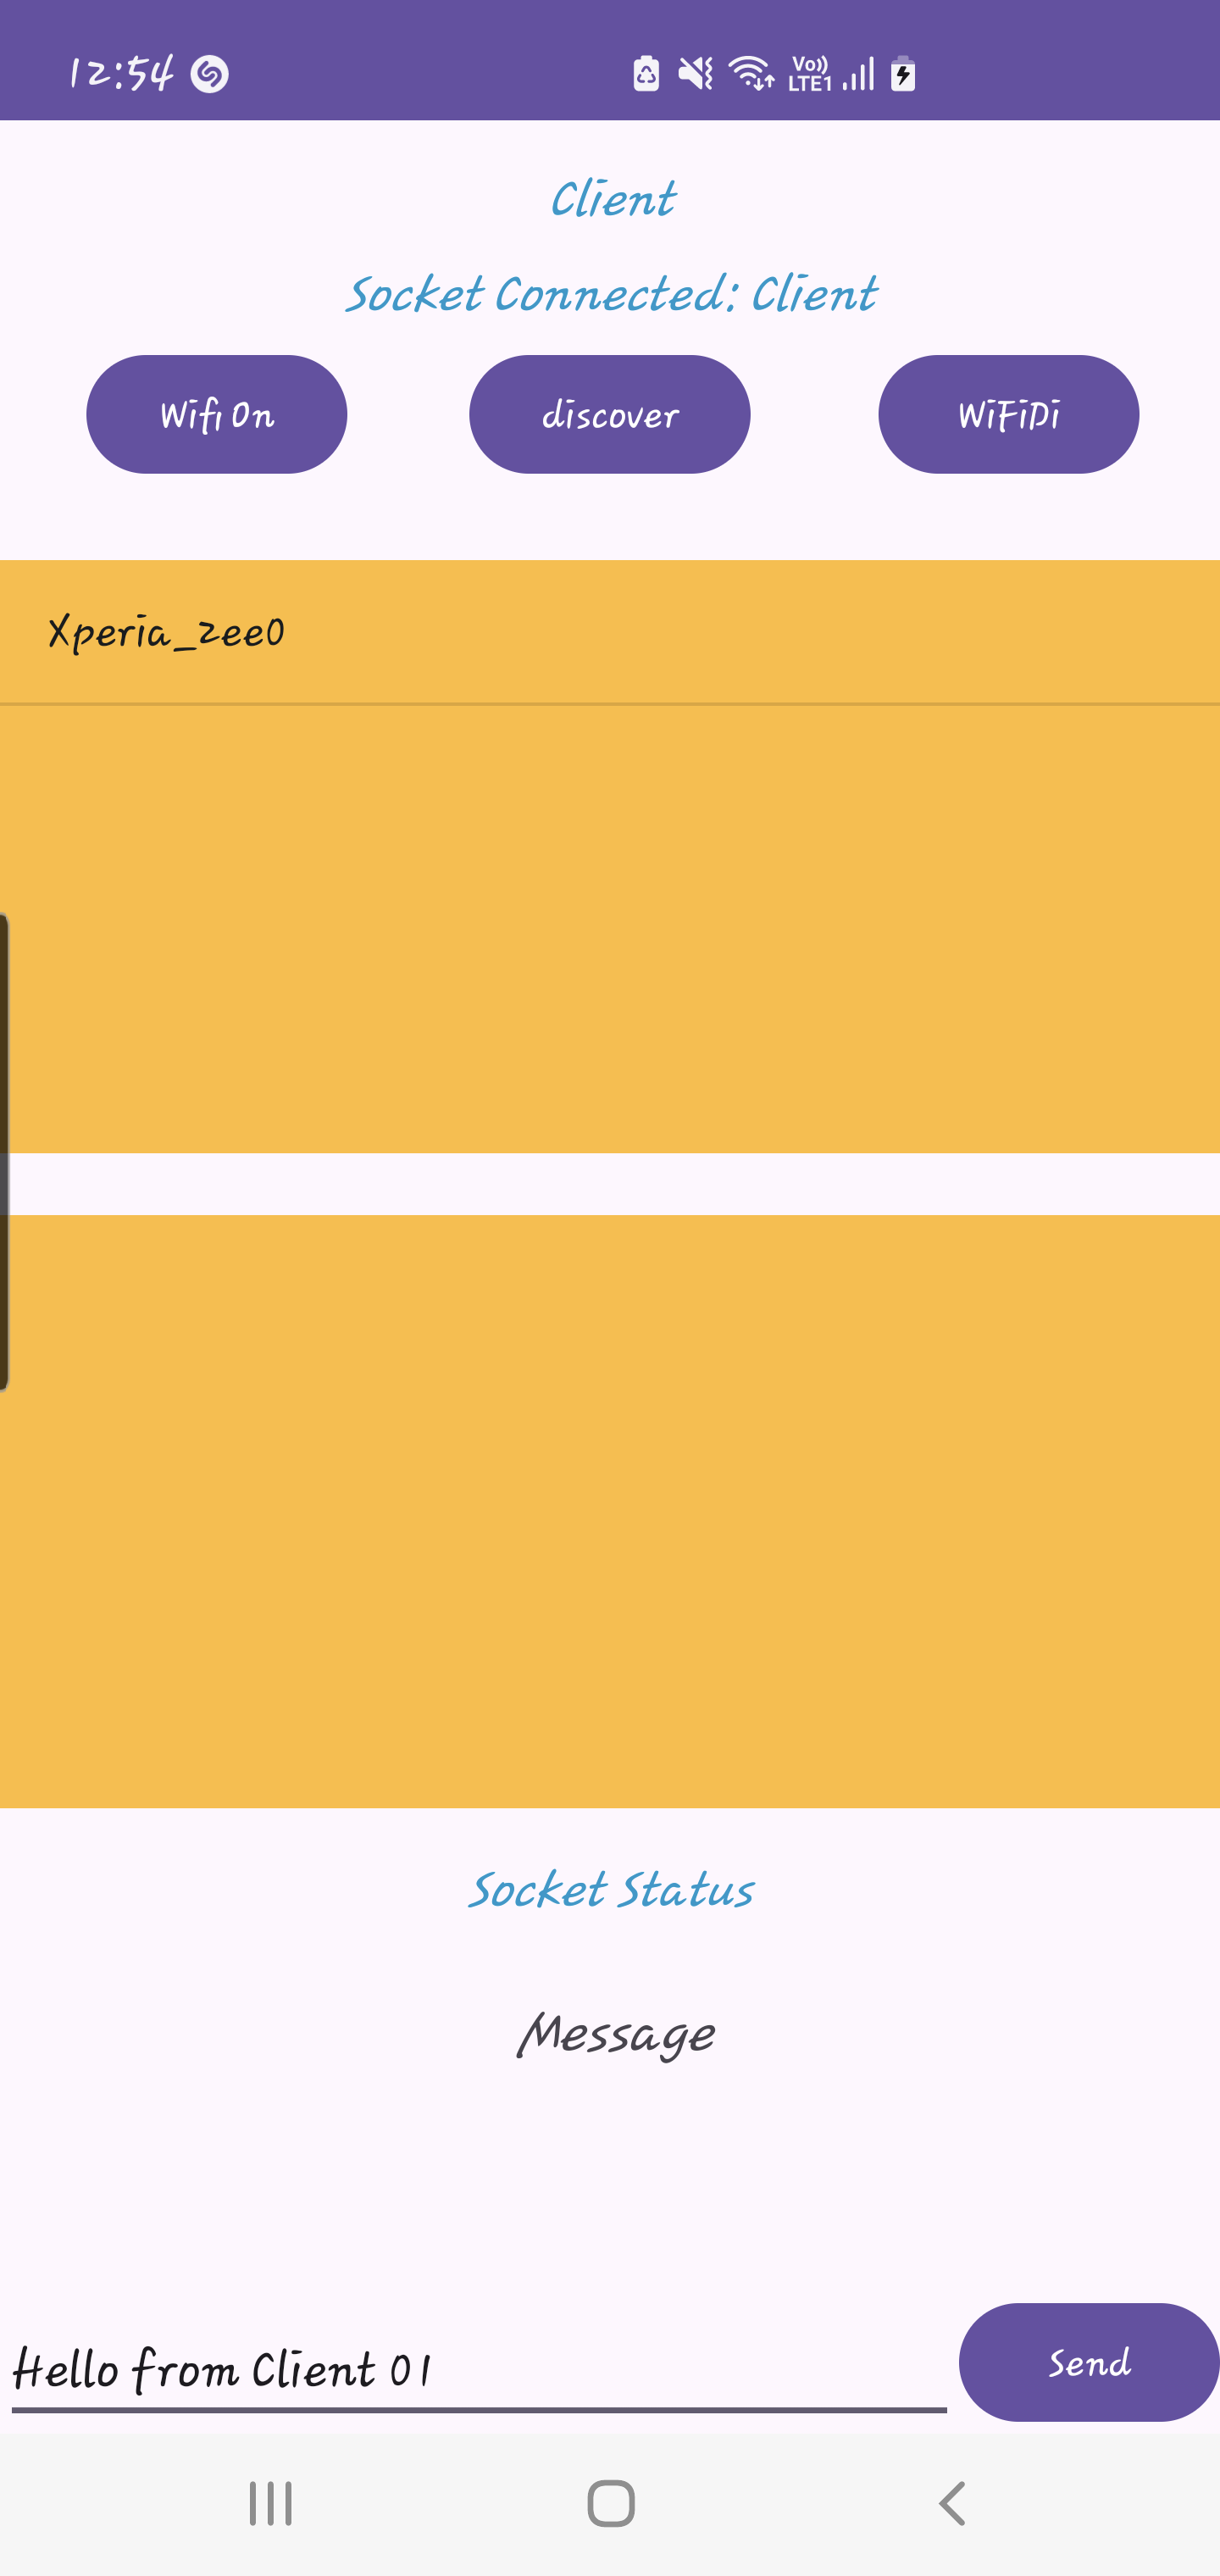
\includegraphics[width=\textwidth,
                height=0.4\textheight]{imgs/client2host-client.png}}
        \caption{Client sends a message to host.}
        \label{clientComm:c}
    \end{subfigure}
    \hspace{1cm}
    \begin{subfigure}[b]{0.3\textwidth}
        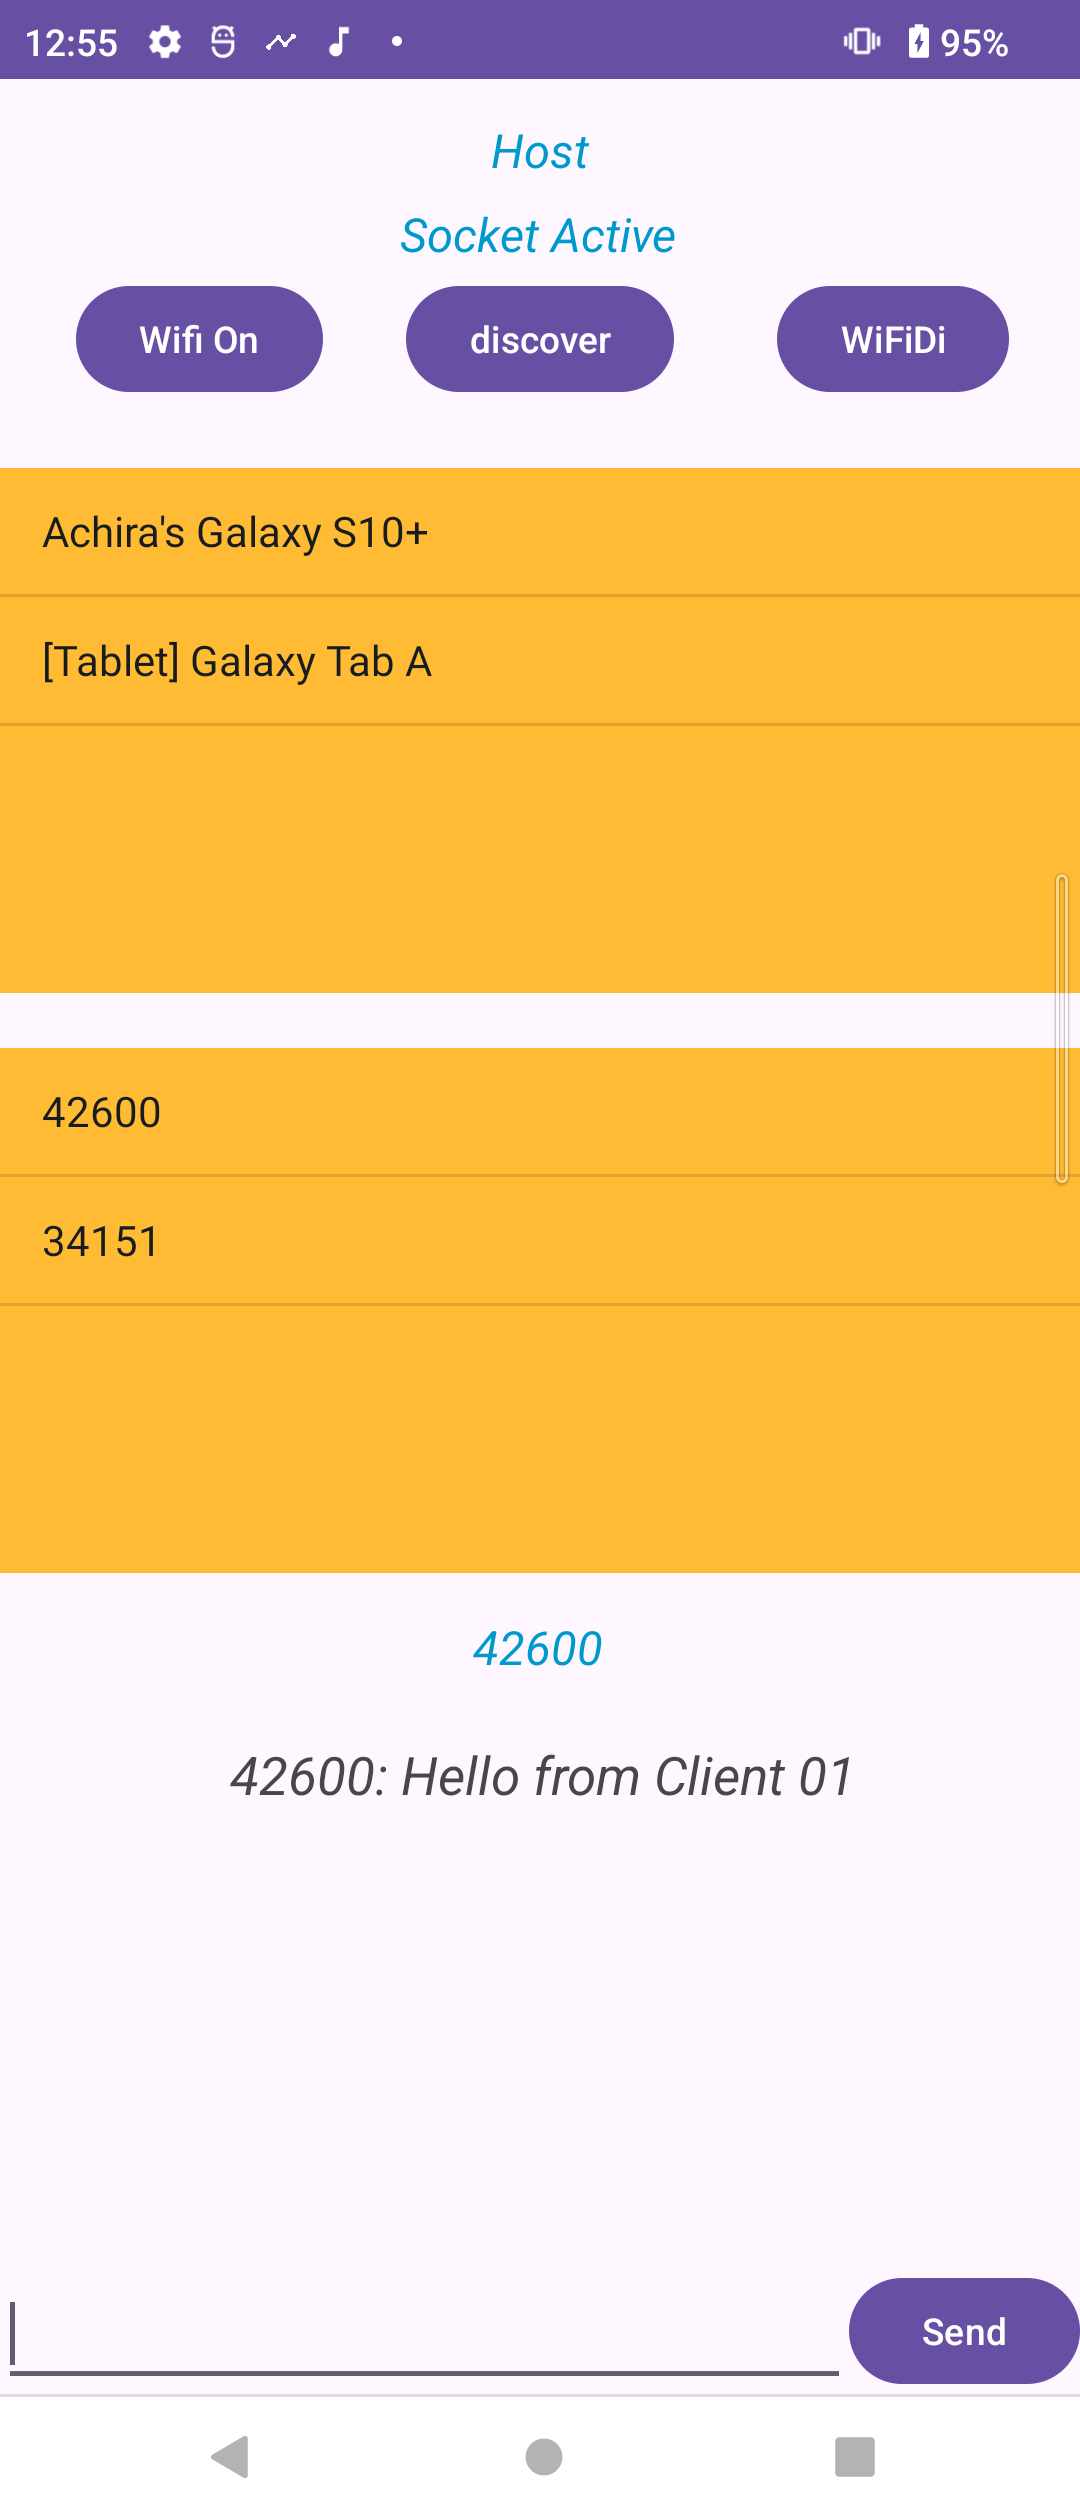
\includegraphics[width=\textwidth,
            height=0.4\textheight]{imgs/client2host-host.png}
        \caption{Message is recieved by host.}
        \label{clientComm:h}
    \end{subfigure}
    \caption{Sending messages from Client to Host.}
    \label{clientComm}
\end{figure}

\begin{figure}
    \centering
    \begin{subfigure}[b]{0.3\textwidth}
        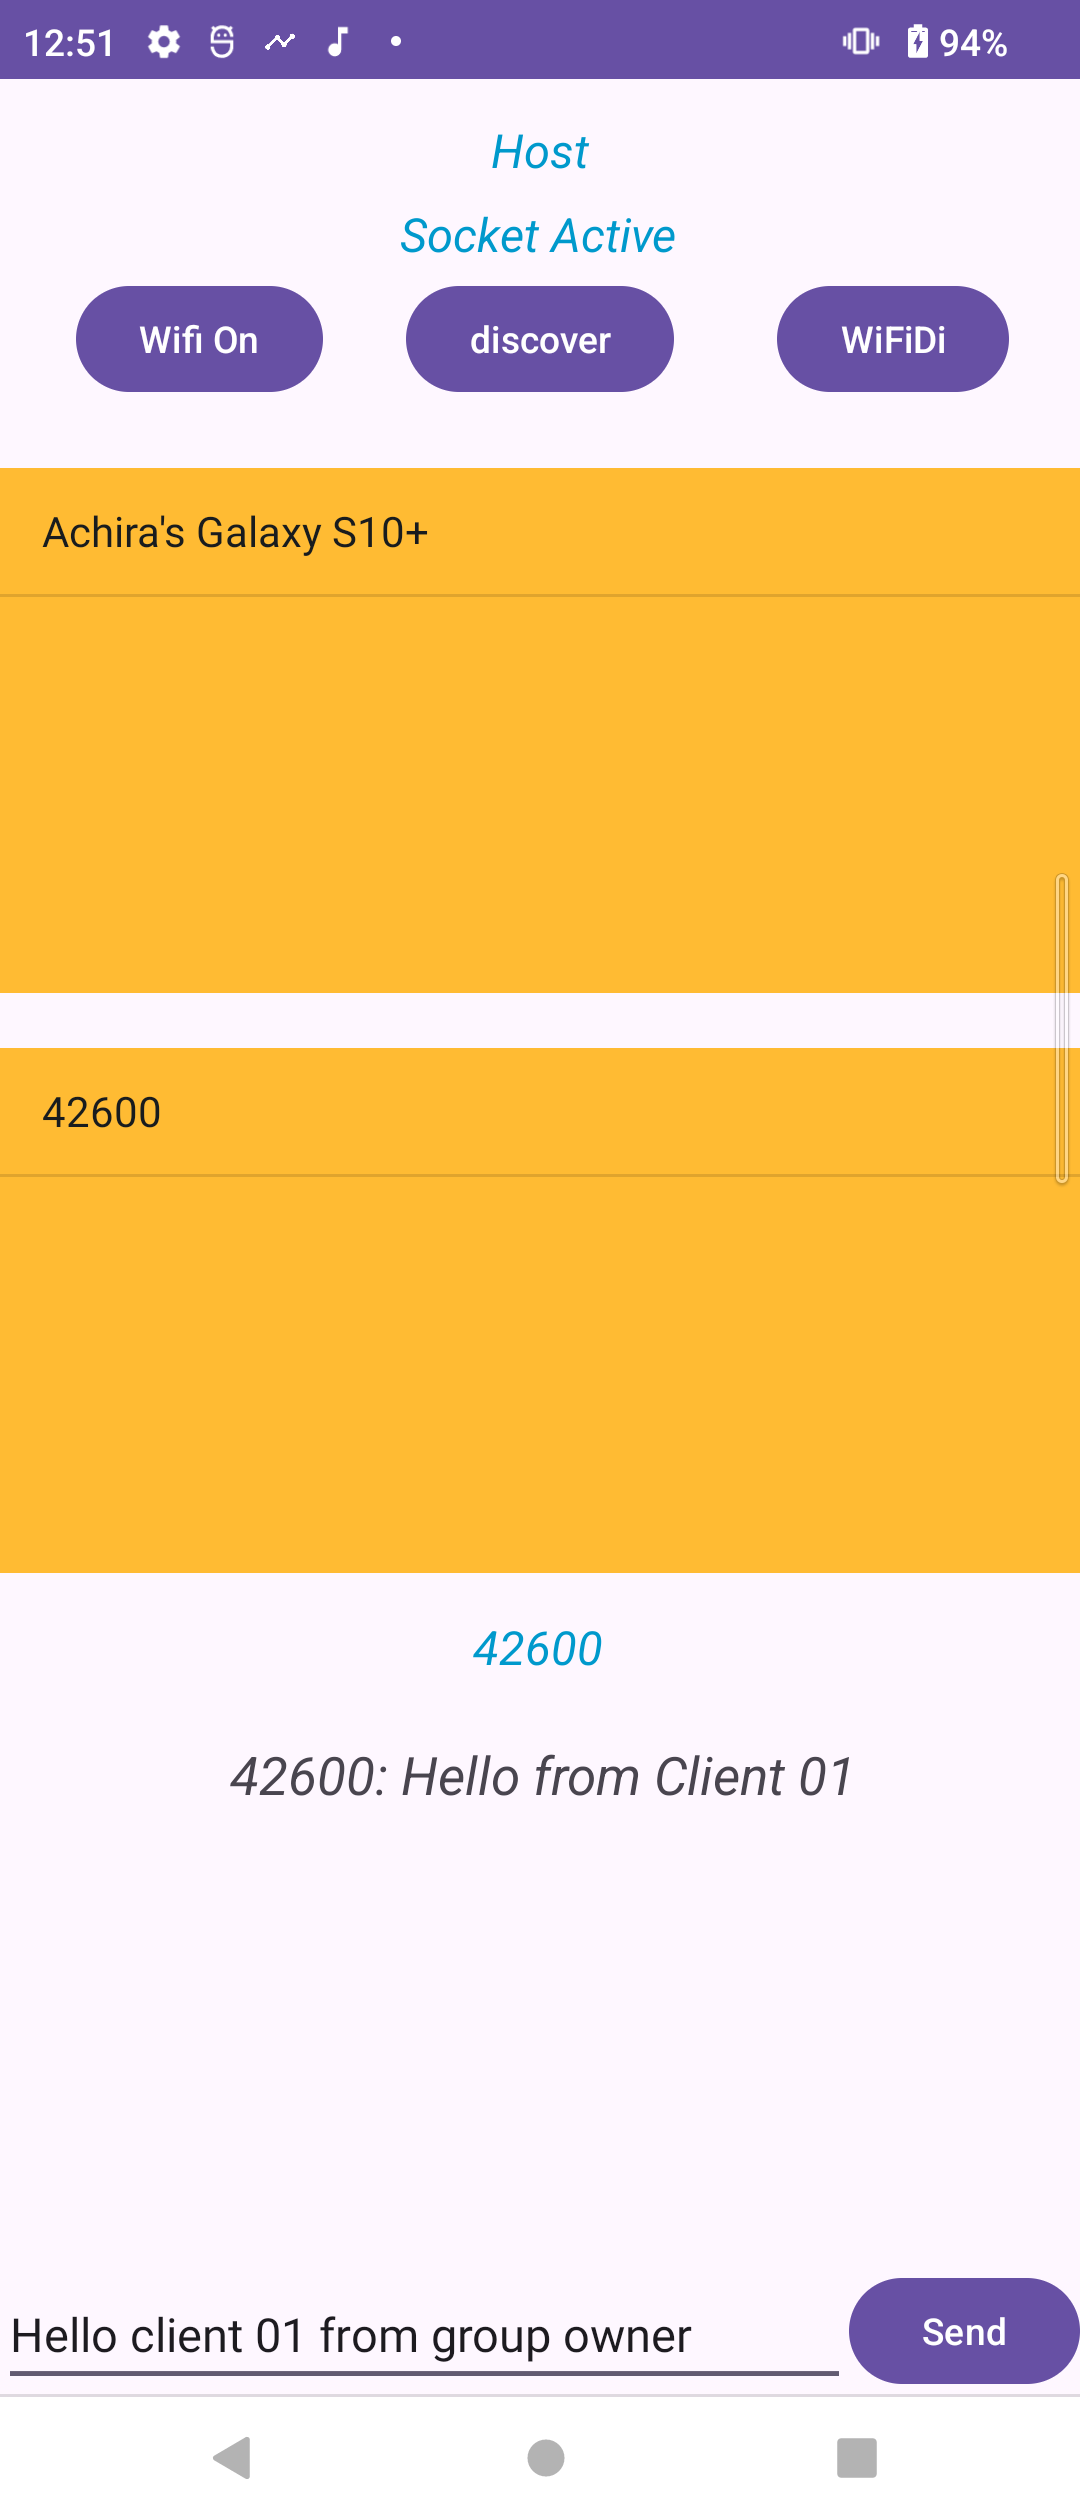
\includegraphics[width=\textwidth,
            height=0.4\textheight]{imgs/host2client-host.png}
        \caption{Host sends a message to client.}
        \label{hostComm:h}
    \end{subfigure}
    \hspace{1cm}
    \begin{subfigure}[b]{0.3\textwidth}
        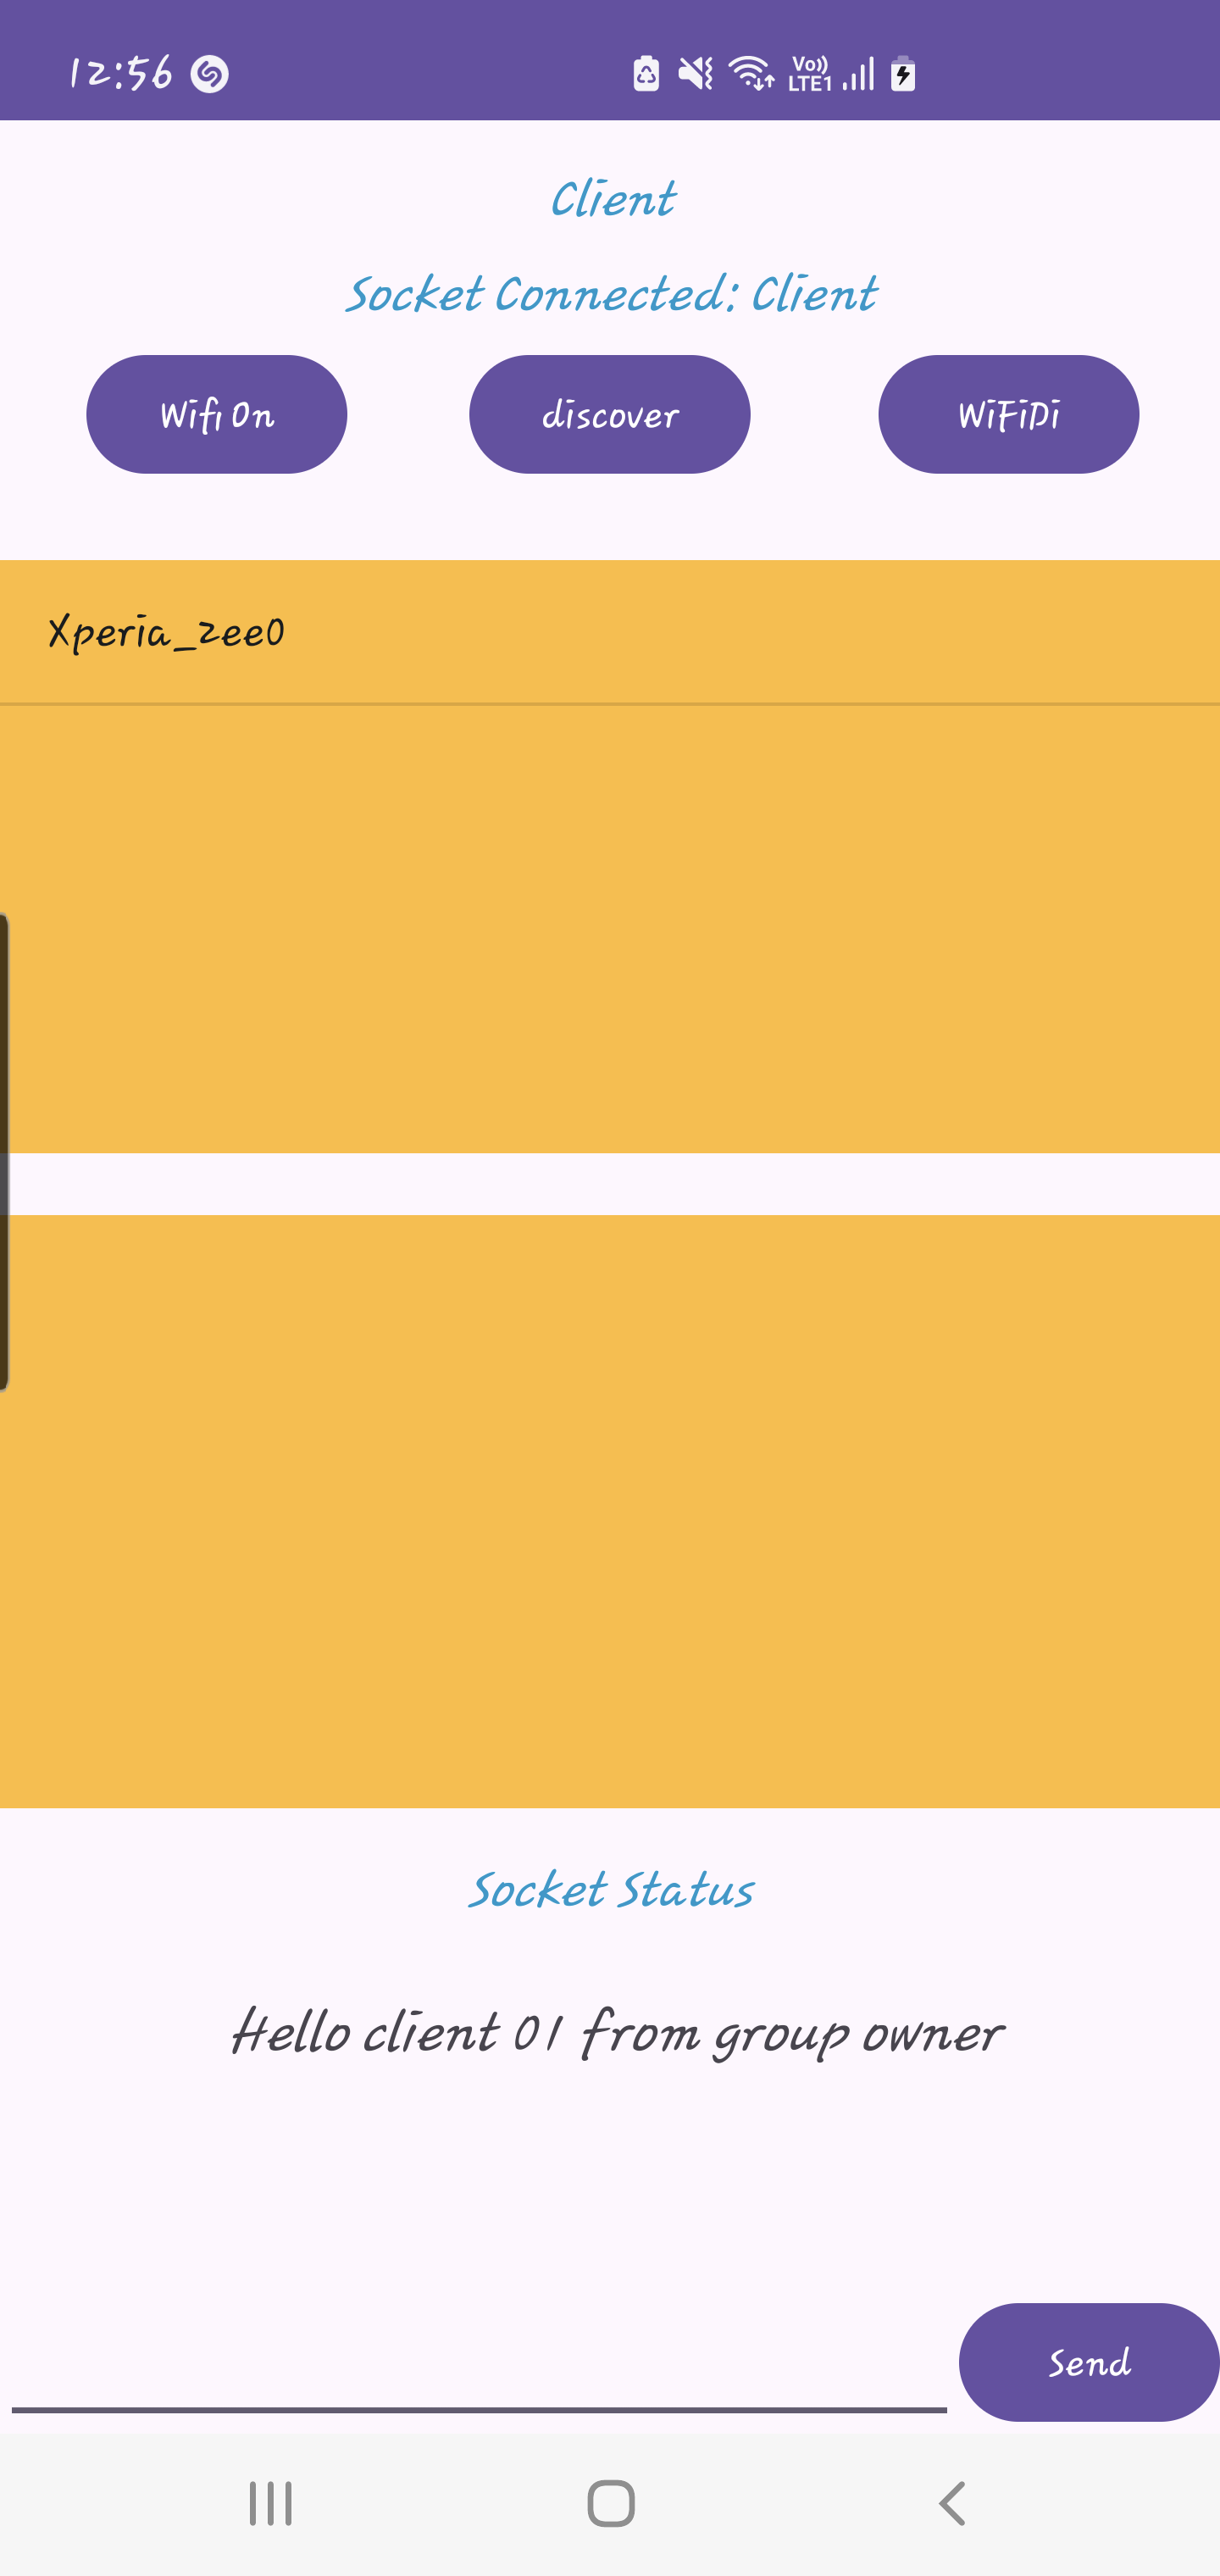
\includegraphics[width=\textwidth,
            height=0.4\textheight]{imgs/host2client-client.png}
        \caption{Message is received by client.}
        \label{hostComm:c}
    \end{subfigure}
    \caption{Sending messages from Host to Client.}
    \label{hostComm}
\end{figure}

It is also possible for another device to connect to an already-established
Group. In such a case, the join request will be approved by the Group Owner.
This is demonstrated by the Figure~\ref{newClient}.

\begin{figure}
    \centering
    \begin{subfigure}[b]{0.6\textwidth}
        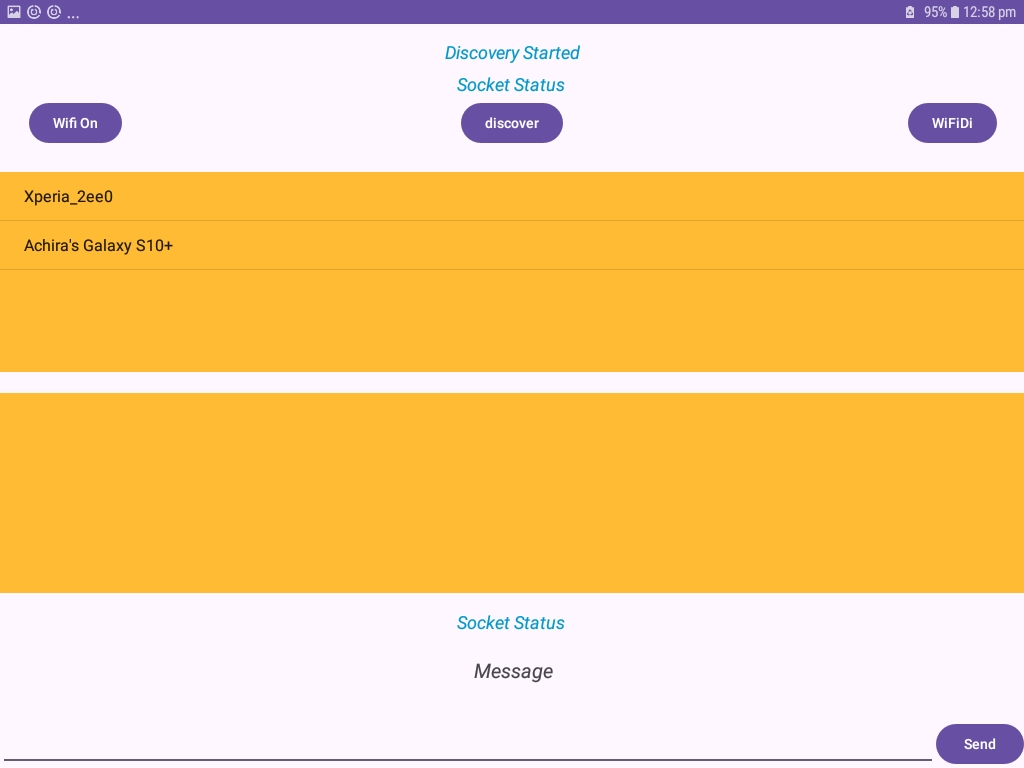
\includegraphics[width=\textwidth,
            height=0.4\textheight]{imgs/discovery-newclient.jpg}
        \caption{A new client is in discovery mode within range of the existing
            group owner}
        \label{newClient:discover}
    \end{subfigure}
    \hspace{1cm}
    \begin{subfigure}[b]{0.3\textwidth}
        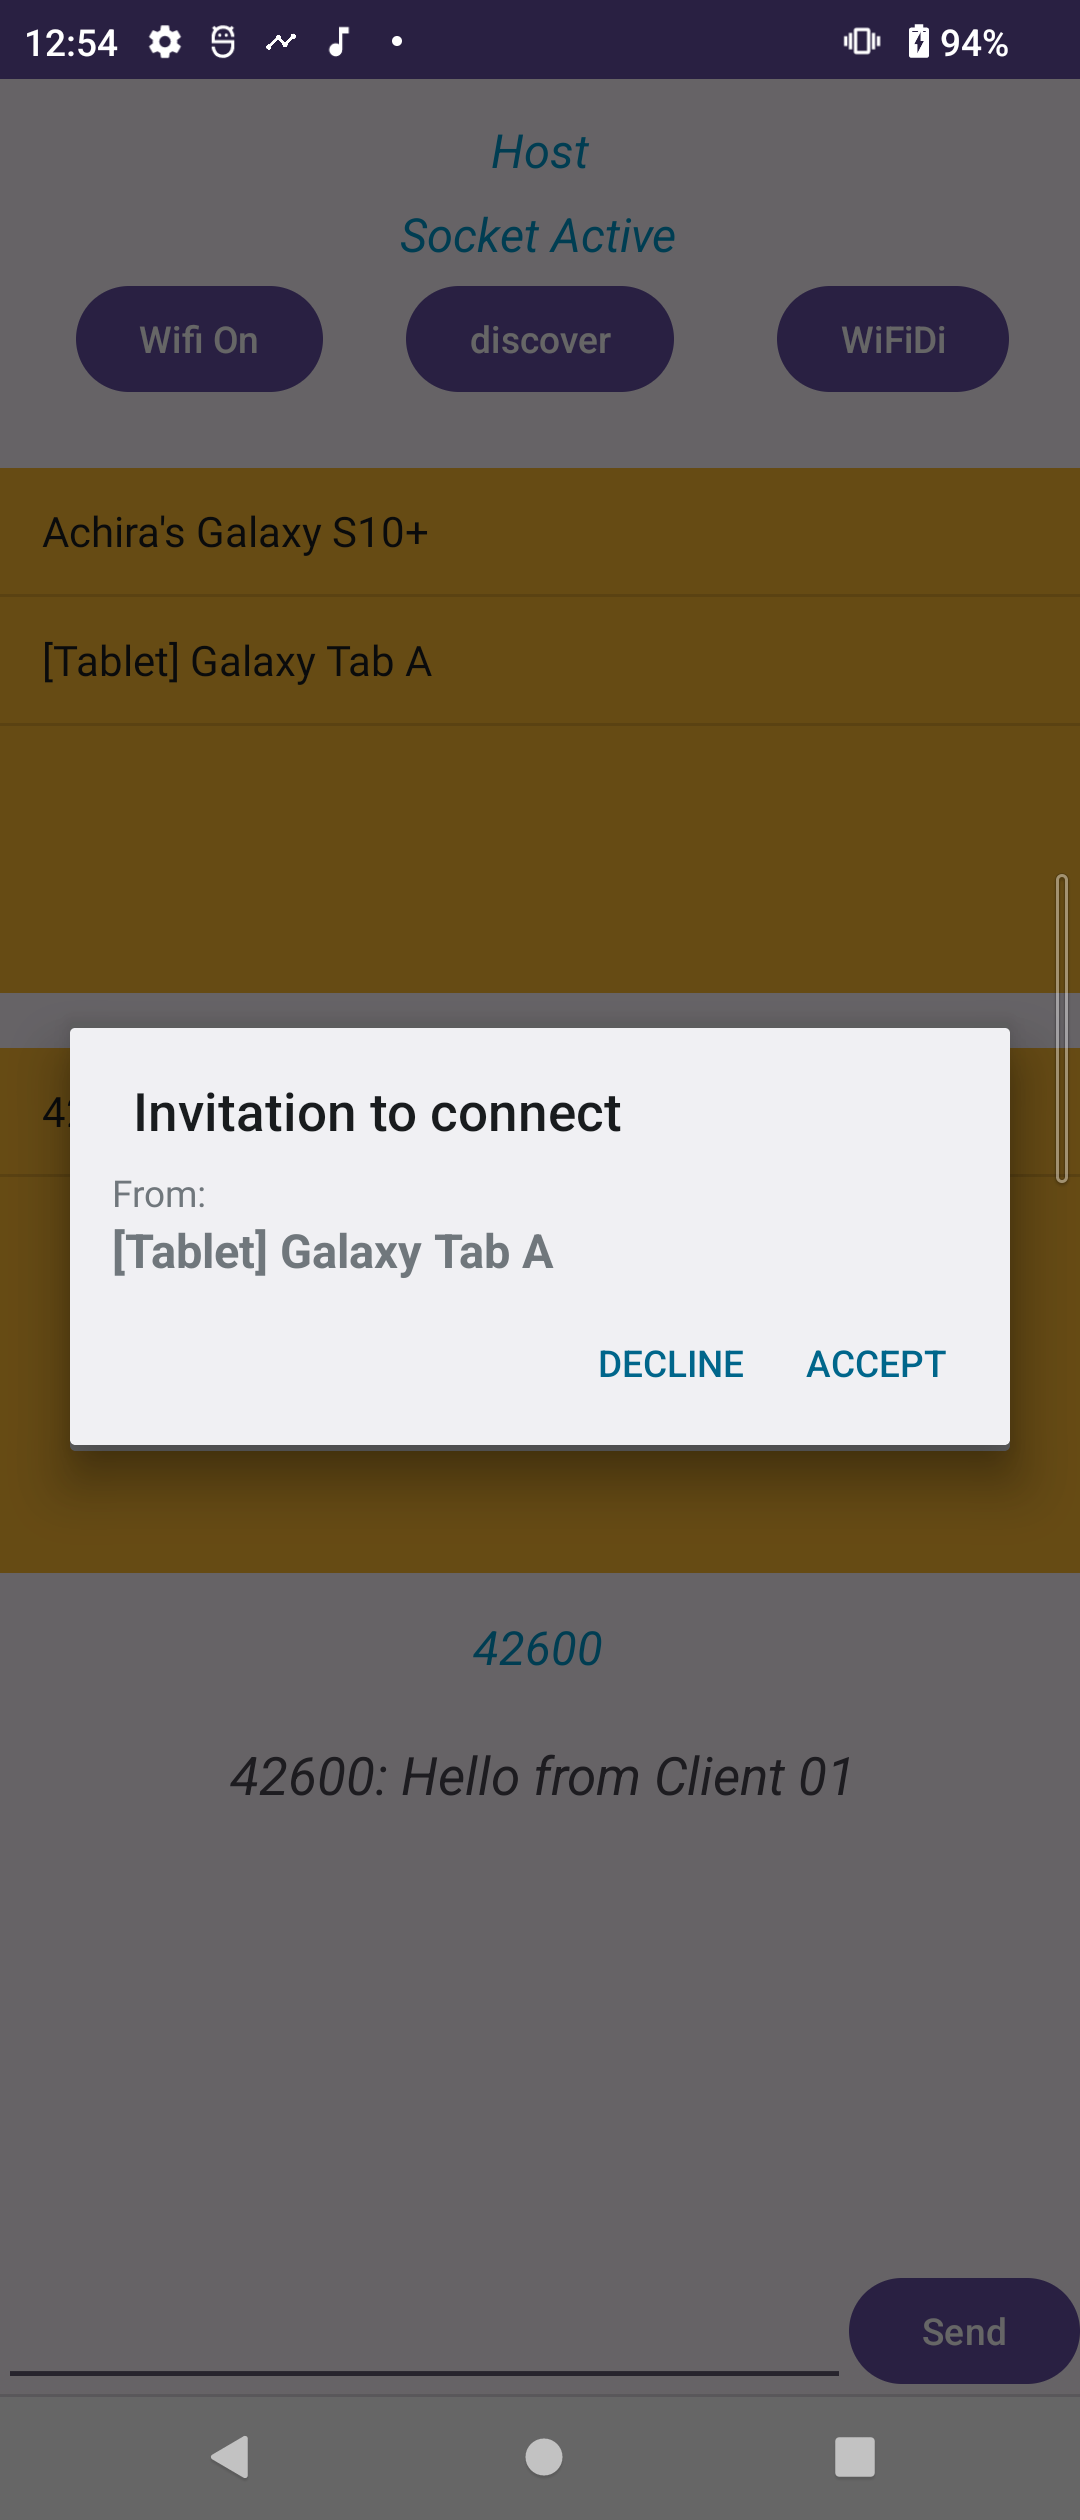
\includegraphics[width=\textwidth,
            height=0.4\textheight]{imgs/newdevice-host.png}
        \caption{Host recieves an incoming connection request from new client.}
        \label{newClient:request}
    \end{subfigure}
    \hspace{1cm}
    \begin{subfigure}[b]{0.6\textwidth}
        \includegraphics[width=\textwidth,
            height=0.4\textheight]{imgs/newClientConnected.jpg}
        \caption{The new client is connected to the group}
        \label{newClient:connected}
    \end{subfigure}
    \caption{Connecting a new client to the existing WiFiDi group}
    \label{newClient}
\end{figure}

Client to client communication is also possible. Such messages will be routed
by the Group Owner. This is demonstrated by Figure~\ref{c2c}.

\begin{figure}
    \centering
    \begin{subfigure}[b]{0.6\textwidth}
        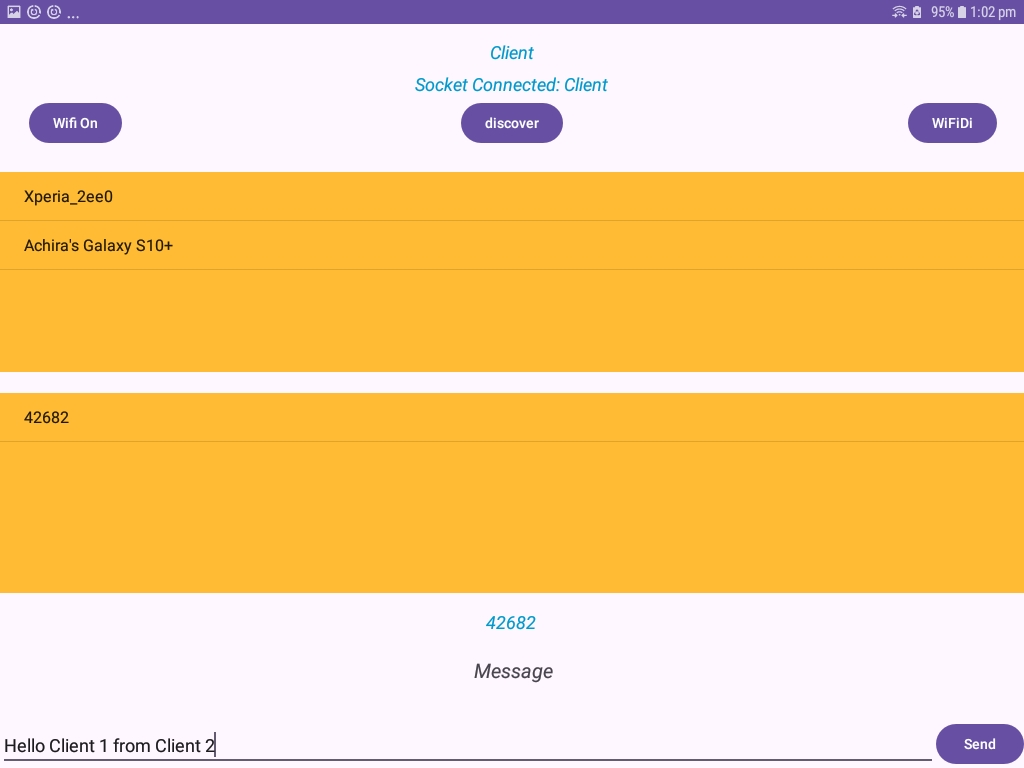
\includegraphics[width=\textwidth,
            height=0.4\textheight]{imgs/client2client-client2.jpg}
        \caption{New client sends a message to \texttt{Client 01}.}
        \label{c2c:1}
    \end{subfigure}
    \hspace{1cm}
    \begin{subfigure}[b]{0.3\textwidth}
        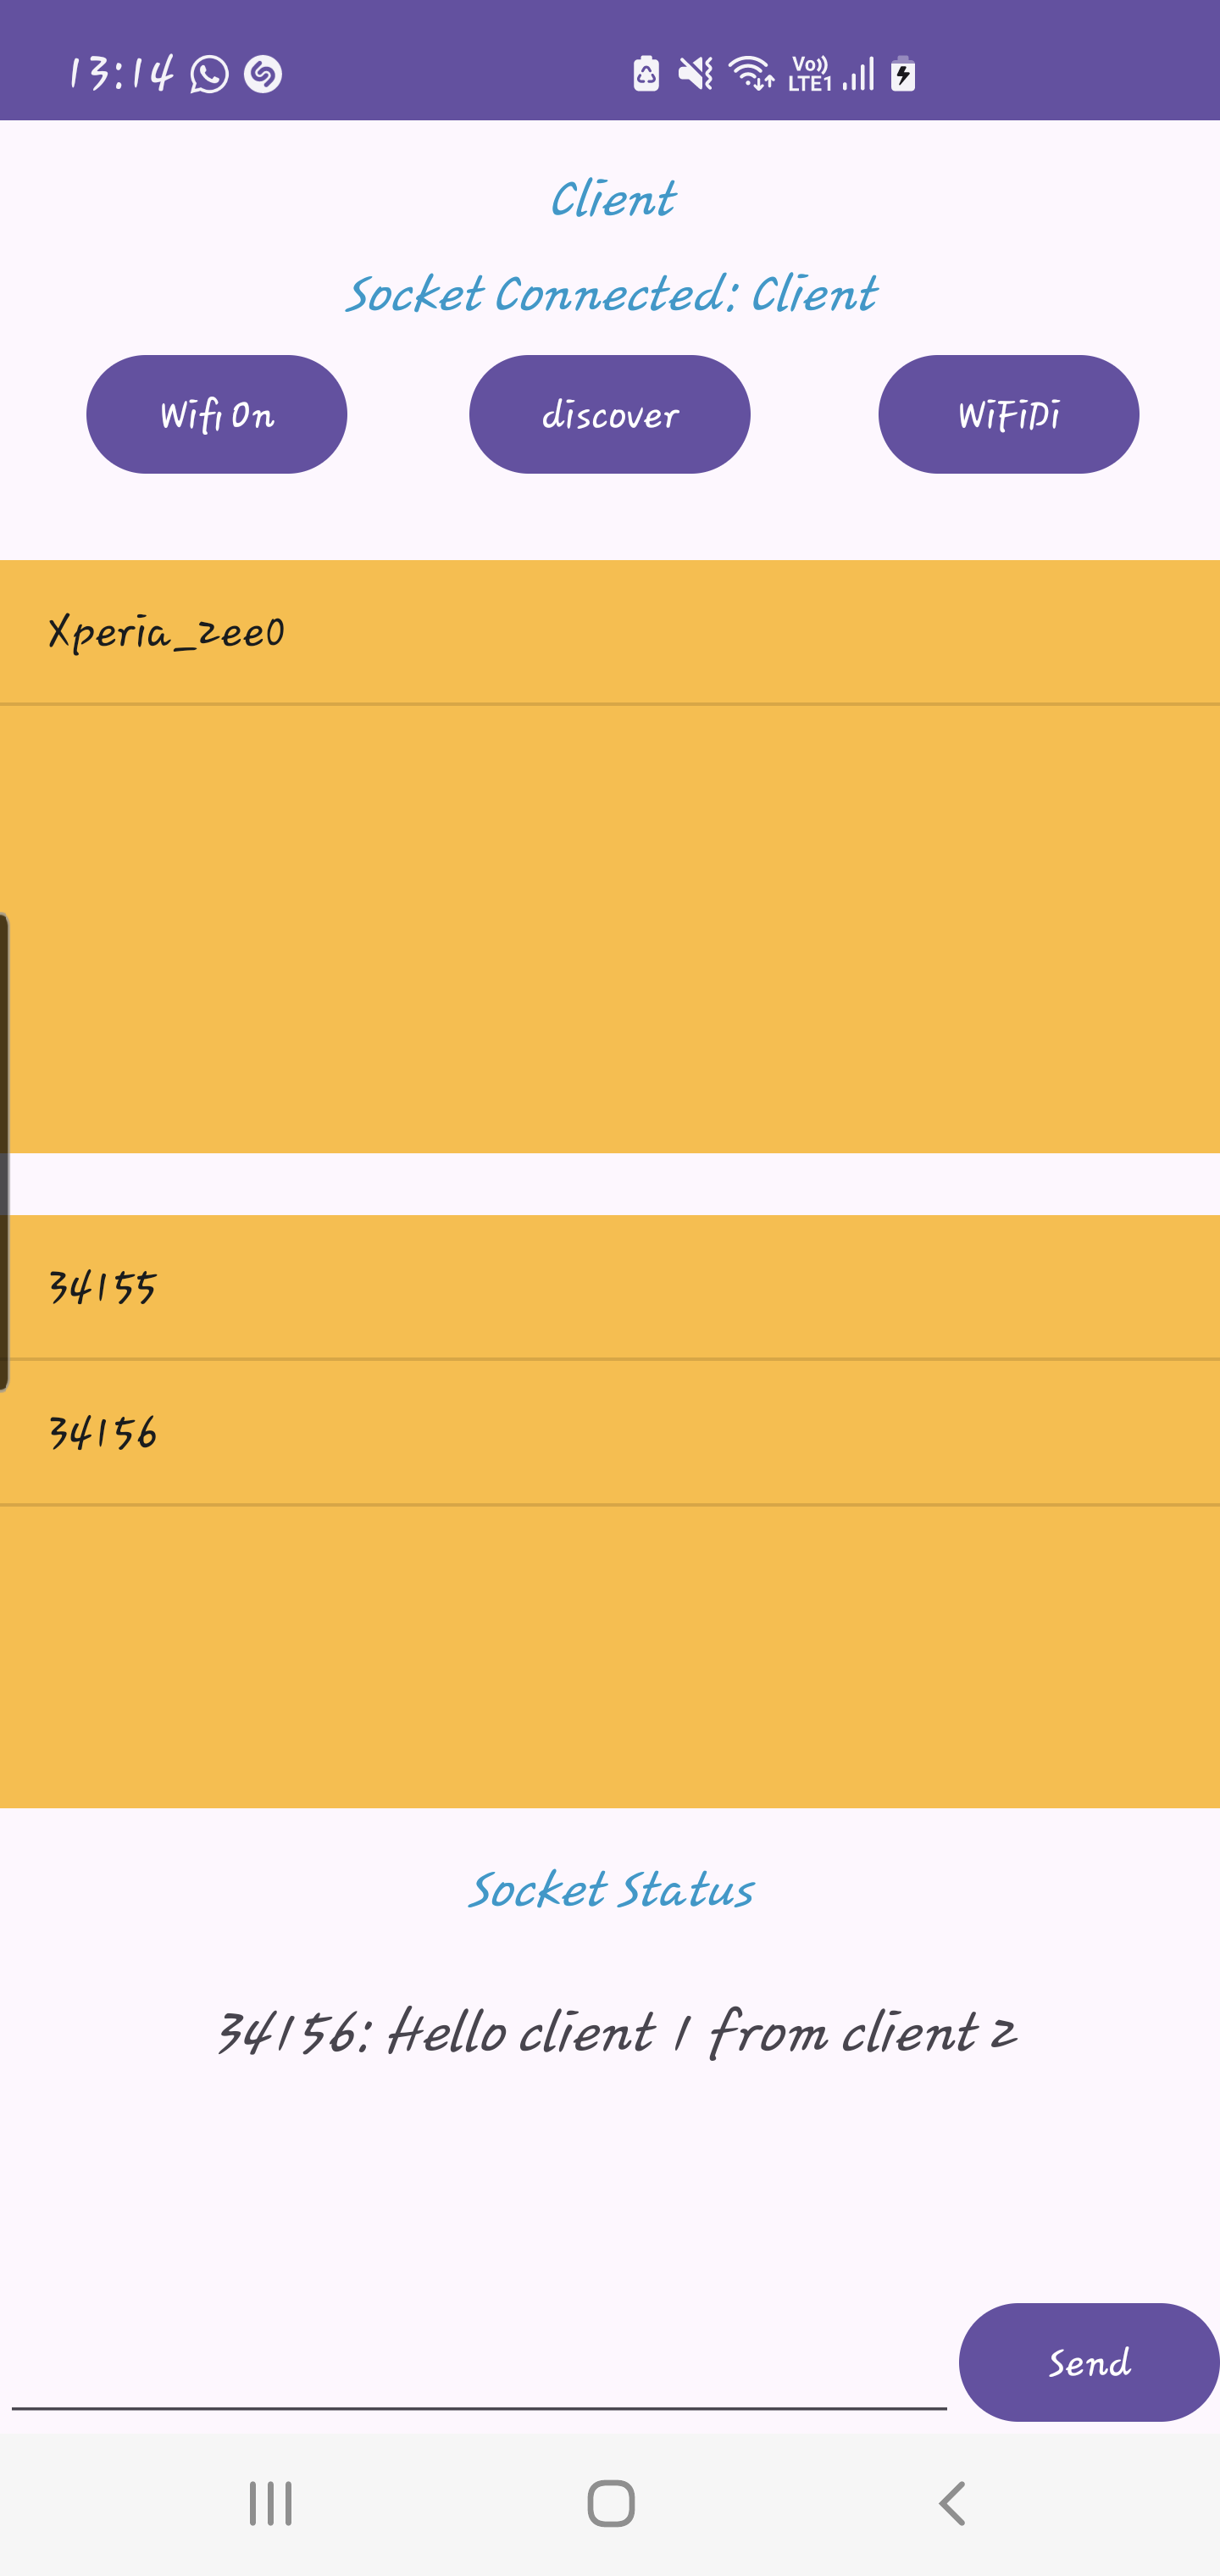
\includegraphics[width=\textwidth,
            height=0.4\textheight]{imgs/client2client-client1.png}
        \caption{Message is recieved by \texttt{Client 01}.}
        \label{c2c:2}
    \end{subfigure}
    \caption{Sending messages from Client to Client.}
    \label{c2c}
\end{figure}

\subsubsection{Improving the framework from Meshify}

Previously the app and the Meshify framework were built in the same project.
Built the framework as a different library project from scratch based on the
previous Meshify framework. The framework supports Bluetooth and BLE.
Framework mainly consists of three sections which are API, Controller and the
Entity. API consists of the main APIs for the framework, Controller consists of
the logic behind the framework where all the above-discussed techniques
including the flooding mechanism with TARP are implemented and Entity
constitutes the foundation for data representation and manipulation within the
Meshify framework. The framework is reusable and modular, allowing its
integration into different applications. All the classes and functionalities of
the framework have been documented for clarification and ease of use.

\vspace{0.3cm}

\subsubsection{Test App for Bluetooth and BLE}

The test app designed to evaluate the framework revealed successful performance
across the following Bluetooth functionalities:

\begin{itemize}
    \item Direct messaging
    \item Multi-hop messaging
    \item Broadcast messaging
\end{itemize}

\begin{figure}
    \centering
    \begin{subfigure}[b]{0.3\textwidth}
        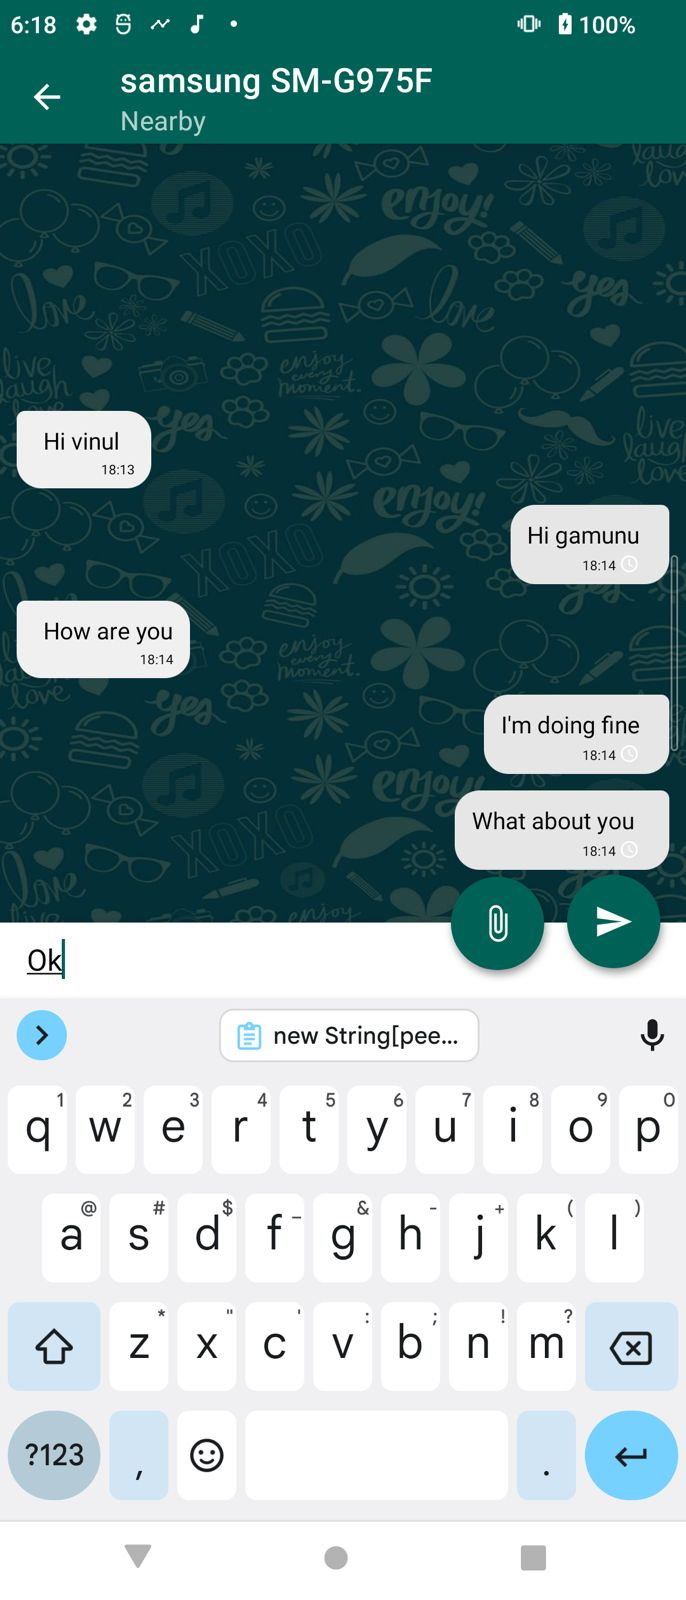
\includegraphics[width=\textwidth,
            height=0.4\textheight]{imgs/dm1.jpeg}
        %\caption{New client sends a message to \texttt{Client 01}.}
        \label{dm:1}
    \end{subfigure}
    \hspace{1cm}
    \begin{subfigure}[b]{0.3\textwidth}
        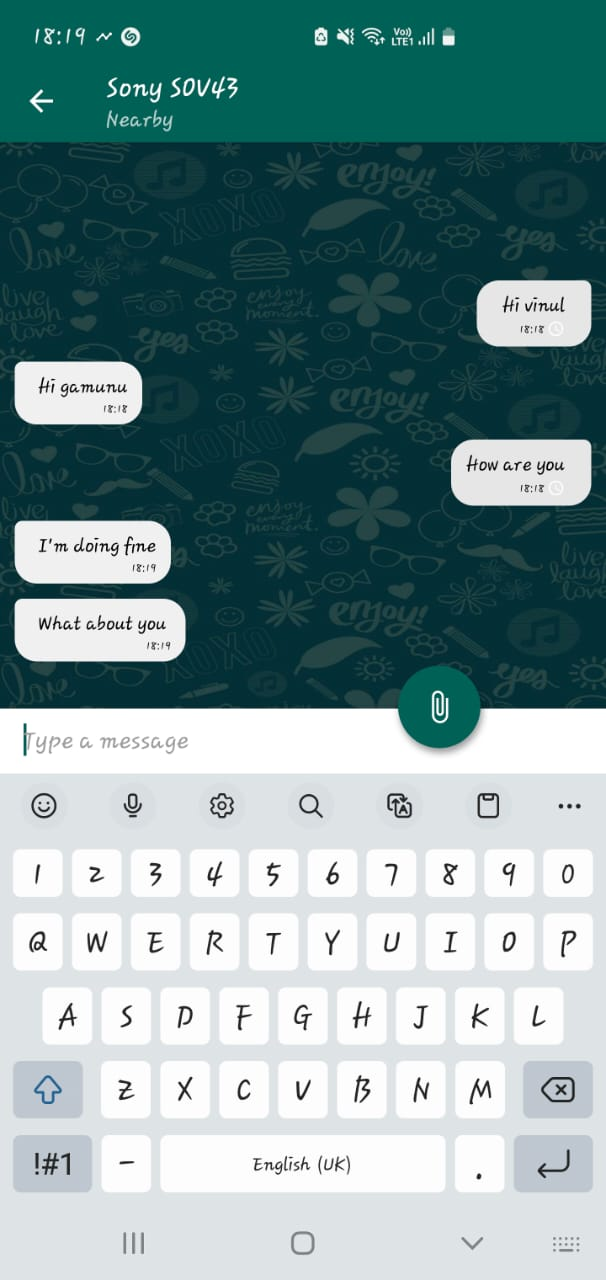
\includegraphics[width=\textwidth,
            height=0.4\textheight]{imgs/dm2.jpeg}
        %\caption{Message is recieved by \texttt{Client 01}.}
        \label{dm:2}
    \end{subfigure}
    \caption{A direct message conversation among two devices.}
    \label{dm}
\end{figure}

\begin{figure}
    \centering
    \begin{subfigure}[b]{0.3\textwidth}
        
\includegraphics[width=\textwidth,
            height=0.4\textheight]{imgs/broad1.jpeg}
        %\caption{New client sends a message to \texttt{Client 01}.}
        \label{broad:1}
    \end{subfigure}
    \hspace{1cm}
    \begin{subfigure}[b]{0.3\textwidth}
        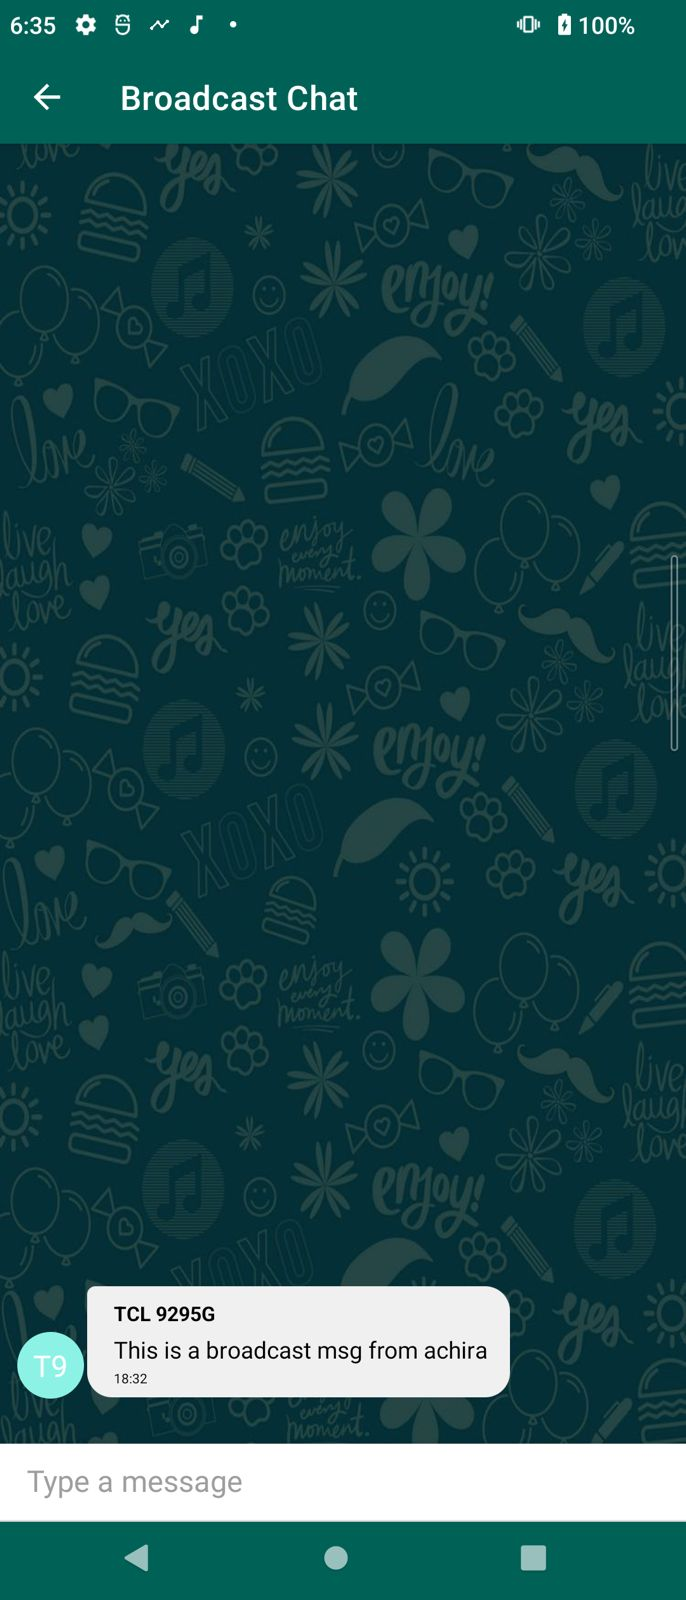
\includegraphics[width=\textwidth,
            height=0.4\textheight]{imgs/broad2.jpeg}
        %\caption{Message is recieved by \texttt{Client 01}.}
        \label{broad:2}
    \end{subfigure}
    \hspace{1cm}
    \begin{subfigure}[b]{0.4\textwidth}
        
\includegraphics[width=\textwidth,
            height=0.4\textheight]{imgs/broad3.jpeg}
        %\caption{Message is recieved by \texttt{Client 01}.}
        \label{broad:3}
    \end{subfigure}
    \caption{Three devices in broadcast messaging.}
    \label{broad}
\end{figure}

Figure~\ref{dm} demonstrates the direct messaging function.
Figure~\ref{broad} demonstrates the broadcast messaging function.

\newpage

\subsection{Upcoming Work}

\subsubsection{Simulation}
\begin{itemize}
    \item Completing the TARP protocol implementation
    \item Performing simulations and analysing data to evaluate relative
          efficiencies of the protocols.
    \item Reporting simulation results in a suitable publication medium.
\end{itemize}

\vspace{0.3cm}

\subsubsection{WiFi Direct POC}
\begin{itemize}
    \item Inter-group communication methods are to be investigated.
    \item Implementation of a selected inter-group communication method.
    \item Formalizing the WiFi Direct functionalities to a framework.
\end{itemize}

\vspace{0.3cm}

\subsubsection{Framework Development}
\begin{itemize}
    \item Integrating WIFI-Direct into the framework.
    \item Refining the code structure, including introducing the TARP protocol
          explicitly.
    \item Publishing the framework library to the Maven repository.
    \item Incorporating Bluetooth Low Energy (BLE) functionality into the test
          app and conducting thorough testing to assess the framework's compatibility
          with BLE.
\end{itemize}


\section{Research timeline}

Fig.~\ref{gantt} shows a Gantt chart representing the project timeline.

The legend of the diagram is as follows
\sethlcolor{yellow}
\begin{itemize}
    \item \hl{All}
    \sethlcolor{specBlue}
    \item \hl{Gamunu}
    \sethlcolor{green}
    \item \hl{Achira}
    \sethlcolor{lightcyan}
    \item \hl{Vinul}
\end{itemize}

%[height=0.45\textwidth]
\begin{figure}[htbp]
    \centerline{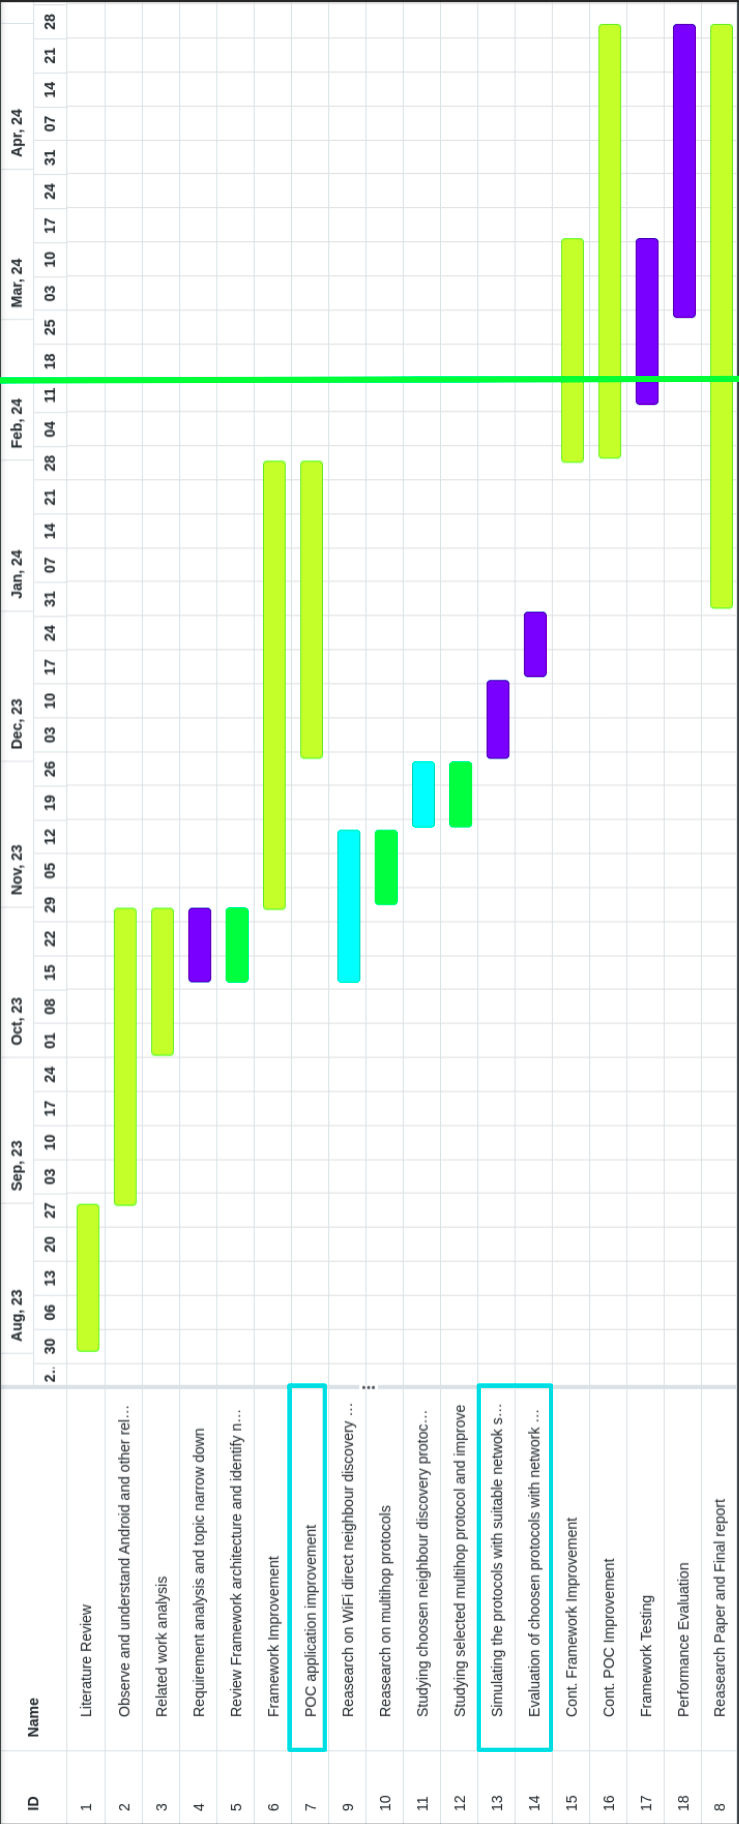
\includegraphics[height=1.4\textwidth]{imgs/gantt.png}}
    \caption{Gantt Chart}
    \label{gantt}
\end{figure}

\newpage
\newpage

\section{Conclusion}

To develop a comprehensive framework that enables users to easily exchange text
messages, media, and various file kinds, the framework will be improved by
adding WiFi Direct as a communication medium, improving BLE capabilities and
the existing protocols. It will enhance adaptability, quickness, and
dependability in various circumstances and settings. The resulting framework
will increase the usability and convenience of the chat application and offer
reusability. With these developments, the project paves the way for better
communication capacities in any environment without infrastructure, providing a
solid answer to users' changing needs.

% \begin{thebibliography}{00}
%     \bibitem{b1} G. Eason, B. Noble, and I. N. Sneddon, ``On certain integrals
%     of
%     Lipschitz-Hankel type involving products of Bessel functions,'' Phil.
%     Trans.
%     Roy. Soc. London, vol. A247, pp. 529--551, April 1955.
%     \bibitem{b2} J. Clerk Maxwell, A Treatise on Electricity and Magnetism, 3rd
%     ed., vol. 2. Oxford: Clarendon, 1892, pp.68--73.
%     \bibitem{b3} I. S. Jacobs and C. P. Bean, ``Fine particles, thin films and
%     exchange anisotropy,'' in Magnetism, vol. III, G. T. Rado and H. Suhl, Eds.
%     New
%     York: Academic, 1963, pp. 271--350.
%     \bibitem{b4} K. Elissa, ``Title of paper if known,'' unpublished.
%     \bibitem{b5} R. Nicole, ``Title of paper with only first word
%     capitalized,'' J.
%     Name Stand. Abbrev., in press.
%     \bibitem{b6} Y. Yorozu, M. Hirano, K. Oka, and Y. Tagawa, ``Electron
%     spectroscopy studies on magneto-optical media and plastic substrate
%     interface,'' IEEE Transl. J. Magn. Japan, vol. 2, pp. 740--741, August 1987
%         [Digests 9th Annual Conf. Magnetics Japan, p. 301, 1982].
%     \bibitem{b7} M. Young, The Technical Writer's Handbook. Mill Valley, CA:
%     University Science, 1989.
% \end{thebibliography}

% \bibliography{proposal}
% \bibliographystyle{ieeetr}

% \begin{thebibliography}{10}

%     \bibitem{akyildiz2002}
%     I.~Akyildiz, W.~Su, Y.~Sankarasubramaniam, and E.~Cayirci, ``Wireless
%     sensor
%     networks: a survey,'' {\em Computer Networks}, vol.~38, pp.~393--422, 3
%     2002.

%     \bibitem{chlamtac2003}
%     I.~Chlamtac, M.~Conti, and J.~J.-N. Liu, ``Mobile ad hoc networking:
%     imperatives and challenges,'' {\em Ad Hoc Networks}, vol.~1, pp.~13--64,
%     7
%     2003.

%     \bibitem{gardner2013}
%     P.~Gardner-Stephen, R.~Challans, J.~Lakeman, A.~Bettison,
%     D.~Gardner-Stephen,
%     and M.~Lloyd, ``The serval mesh: A platform for resilient communications
%     in
%     disaster and crisis,'' pp.~162--166, IEEE, 10 2013.

%     \bibitem{meshrabiya}
%     M.~Dawson, ``Meshrabiya ad hoc networking framework.''

%     \bibitem{bridgefy}
%     ``Bridgefy,'' 2022.

%     \bibitem{todtenberg2019}
%     N.~Todtenberg and R.~Kraemer, ``A survey on bluetooth multi-hop networks,''
%     {\em Ad Hoc Networks}, vol.~93, 2019.

%     \bibitem{gunasekara2022}
%     K.~Perera, J.~Ranidu, and K.~Gunasekera, ``Towards an adaptive
%     communication
%     framework for smart devices,'' 7 2022.

%     \bibitem{wsn2021}
%     P.~Gburzyński, ``A wsn architecture for building resilient, reactive and
%     secure wireless sensing systems,'' {\em TASK QUARTERLY}, vol.~25,
%     pp.~141--181, 2021.

%     \bibitem{malar2023}
%     A.~C.~J. Malar, R.~Kanmani, M.~D. Priya, G.~Nivedhitha, P.~Divya, and
%     T.~S.~P.
%     Surya, {\em An Infrastructure-Less Communication Platform for Android
%             Smartphones Using Wi-Fi Direct}, pp.~135--145.
%     \newblock 2023.

%     \bibitem{funai2015}
%     C.~Funai, C.~Tapparello, and W.~Heinzelman, ``Supporting multi-hop
%     device-to-device networks through wifi direct multi-group networking,''
%     12
%     2015.

%     \bibitem{wifidispec}
%     W.-F. Alliance, {\em Wi-Fi Direct® Specification}.
%     \newblock WiFi Alliance, 1.9~ed., 2021.

%     \bibitem{wifiman}
%     Google, ``Wifip2pmanager class.''

% \end{thebibliography}

\bibliography{proposal}
\bibliographystyle{IEEEtran}

\end{document}